\documentclass[12pt,a4paper,oneside,openany,oneauthor,masterthesis,deansoffice]{mfipl}

\usepackage{float}
\usepackage{graphicx} % Required for inserting images
\usepackage{clrscode}
\usepackage{latexsym}


\begin{document}

\section*{Zadanie 1 - Splot 2D z sygnałem}


\subsection*{(a) Splot $f * h_1$ oraz $f * h_2$}

Wyniki splotu:
\[
f * h_1 = \begin{pmatrix}
0 & 0 & 0 & 0 & 0 & 0 & 0 \\
0 & 0 & -255 & -255 & -255 & 0 & 0 \\
0 & 0 & 0 & 0 & 0 & 0 & 0 \\
0 & 0 & 0 & 0 & 0 & 0 & 0 \\
0 & 0 & 255 & 255 & 255 & 0 & 0 \\
0 & 0 & 0 & 0 & 0 & 0 & 0 \\
-255 & -255 & -255 & -255 & -255 & -255 & -255
\end{pmatrix}
\]
\[
f * h_2 = \begin{pmatrix}
255 & 255 & 255 & 255 & 255 & 255 & 255 \\
0 & 0 & 0 & 0 & 0 & 0 & 0 \\
0 & 0 & -255 & -255 & -255 & 0 & 0 \\
0 & 0 & 0 & 0 & 0 & 0 & 0 \\
0 & 0 & 0 & 0 & 0 & 0 & 0 \\
0 & 0 & 255 & 255 & 255 & 0 & 0 \\
0 & 0 & 0 & 0 & 0 & 0 & 0
\end{pmatrix}
\]

Oba sploty wykrywają te same krawędzie sygnału, jedynie zlokalizowane w różnych wierszach.

\subsection*{(b) 8-bit vs.\ 32-bit}

\[
(f * h_1)_{8\text{-bit}} = \begin{pmatrix}
0 & 0 & 0 & 0 & 0 & 0 & 0 \\
0 & 0 & 0 & 0 & 0 & 0 & 0 \\
0 & 0 & 0 & 0 & 0 & 0 & 0 \\
0 & 0 & 0 & 0 & 0 & 0 & 0 \\
0 & 0 & 255 & 255 & 255 & 0 & 0 \\
0 & 0 & 0 & 0 & 0 & 0 & 0 \\
0 & 0 & 0 & 0 & 0 & 0 & 0
\end{pmatrix}
\]
\[
(f * h_2)_{8\text{-bit}} = \begin{pmatrix}
255 & 255 & 255 & 255 & 255 & 255 & 255 \\
0 & 0 & 0 & 0 & 0 & 0 & 0 \\
0 & 0 & 0 & 0 & 0 & 0 & 0 \\
0 & 0 & 0 & 0 & 0 & 0 & 0 \\
0 & 0 & 0 & 0 & 0 & 0 & 0 \\
0 & 0 & 255 & 255 & 255 & 0 & 0 \\
0 & 0 & 0 & 0 & 0 & 0 & 0
\end{pmatrix}
\]

W 32-bitach (\texttt{float32}) wynik zachowuje wartości ujemne identyczne jak w (a):
\[
(f * h_1)_{32\text{-bit}} = \begin{pmatrix}
0 & 0 & 0 & 0 & 0 & 0 & 0 \\
0 & 0 & -255 & -255 & -255 & 0 & 0 \\
0 & 0 & 0 & 0 & 0 & 0 & 0 \\
0 & 0 & 0 & 0 & 0 & 0 & 0 \\
0 & 0 & 255 & 255 & 255 & 0 & 0 \\
0 & 0 & 0 & 0 & 0 & 0 & 0 \\
-255 & -255 & -255 & -255 & -255 & -255 & -255
\end{pmatrix}
\]
\[
(f * h_2)_{32\text{-bit}} = \begin{pmatrix}
255 & 255 & 255 & 255 & 255 & 255 & 255 \\
0 & 0 & 0 & 0 & 0 & 0 & 0 \\
0 & 0 & -255 & -255 & -255 & 0 & 0 \\
0 & 0 & 0 & 0 & 0 & 0 & 0 \\
0 & 0 & 0 & 0 & 0 & 0 & 0 \\
0 & 0 & 255 & 255 & 255 & 0 & 0 \\
0 & 0 & 0 & 0 & 0 & 0 & 0
\end{pmatrix}
\]

W 8-bitach (\texttt{uint8}, zakres $[0,255]$) wartości ujemne są obcinane do 0, więc znika połowa krawędzi. Format 32-bitowy zachowuje pełen zakres i odtwarza wynik z (a). Różnica wynika z kwantyzacji typu, nie z samego splotu.

\section*{Zadanie 2 - Filtracja obrazu jądrami $h_a$-$h_d$}

\subsection*{(a) Filtracja obrazu \texttt{skarpetyIPhone.png}}

\begin{figure}[H]
\centering
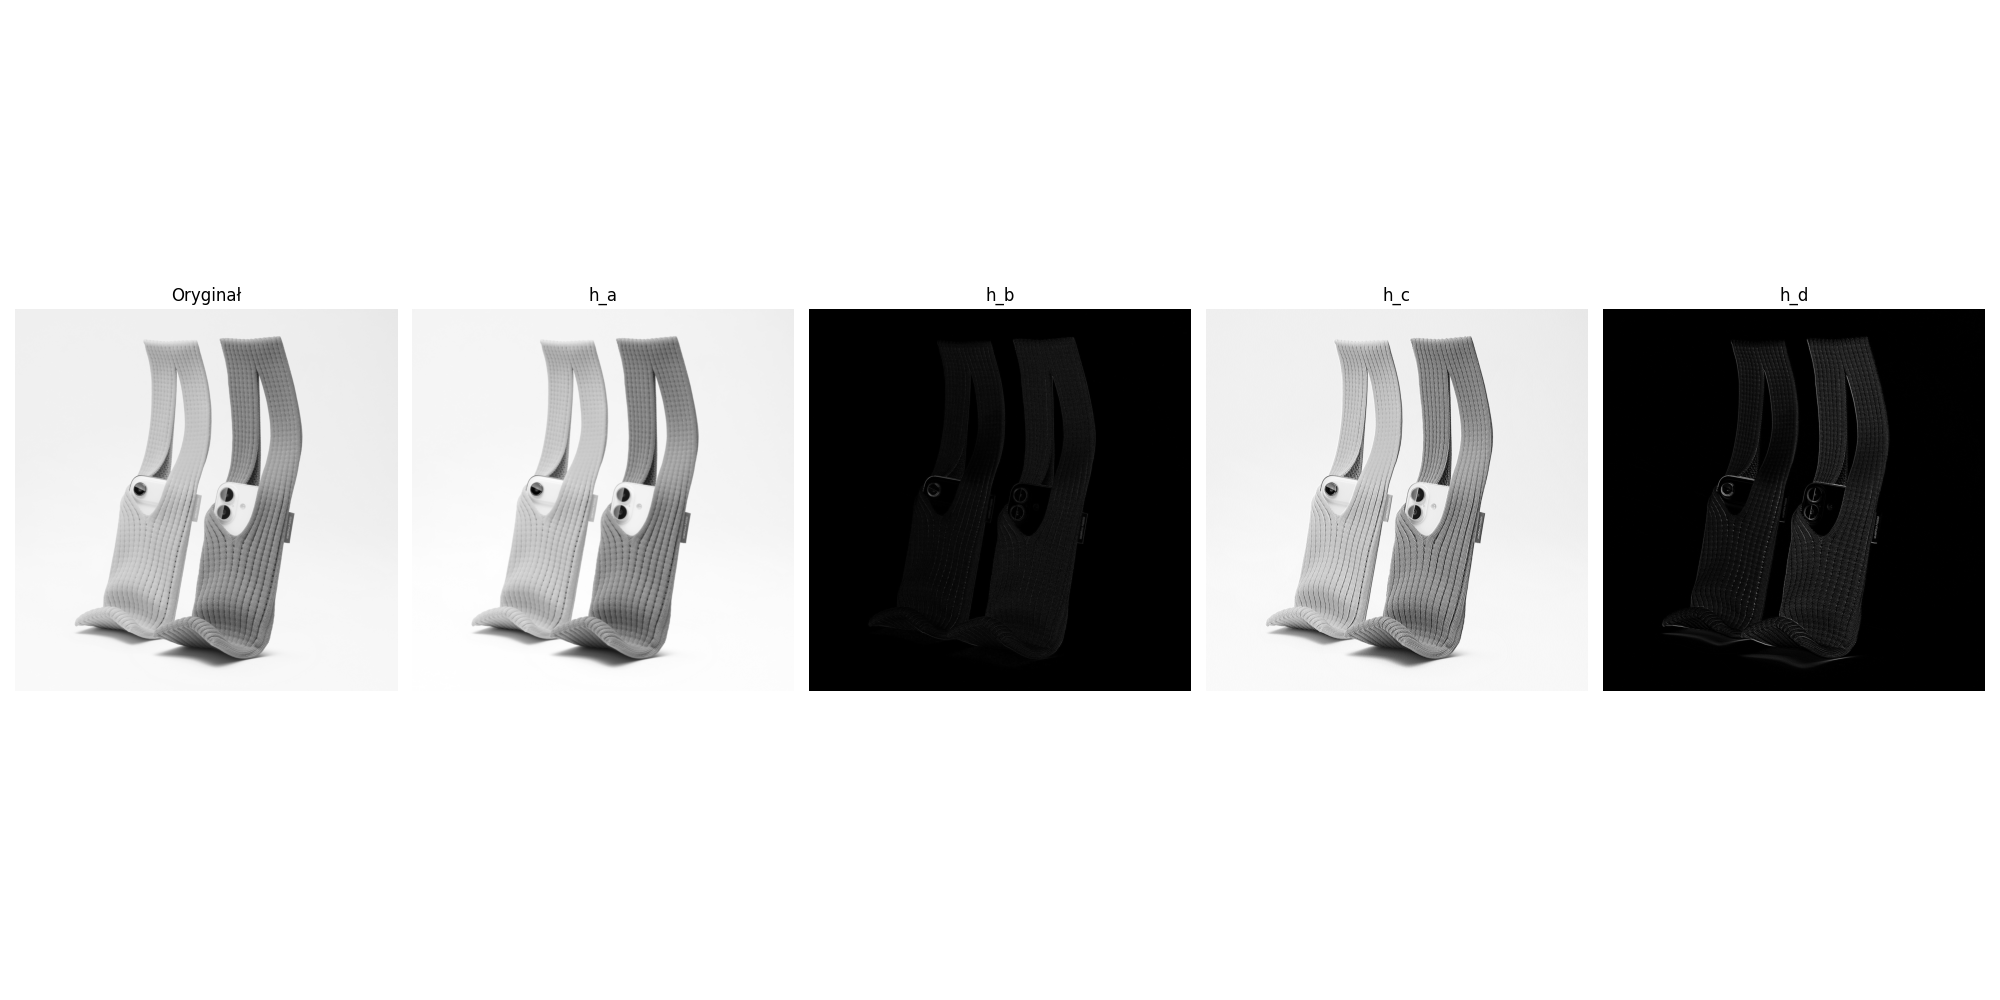
\includegraphics[width=\textwidth]{zad2/zestawienie_filtrowania.png}
\caption{Zestawienie: oryginał oraz wyniki filtracji jądrami $h_a$, $h_b$, $h_c$, $h_d$.}
\end{figure}

\begin{figure}[H]
\centering
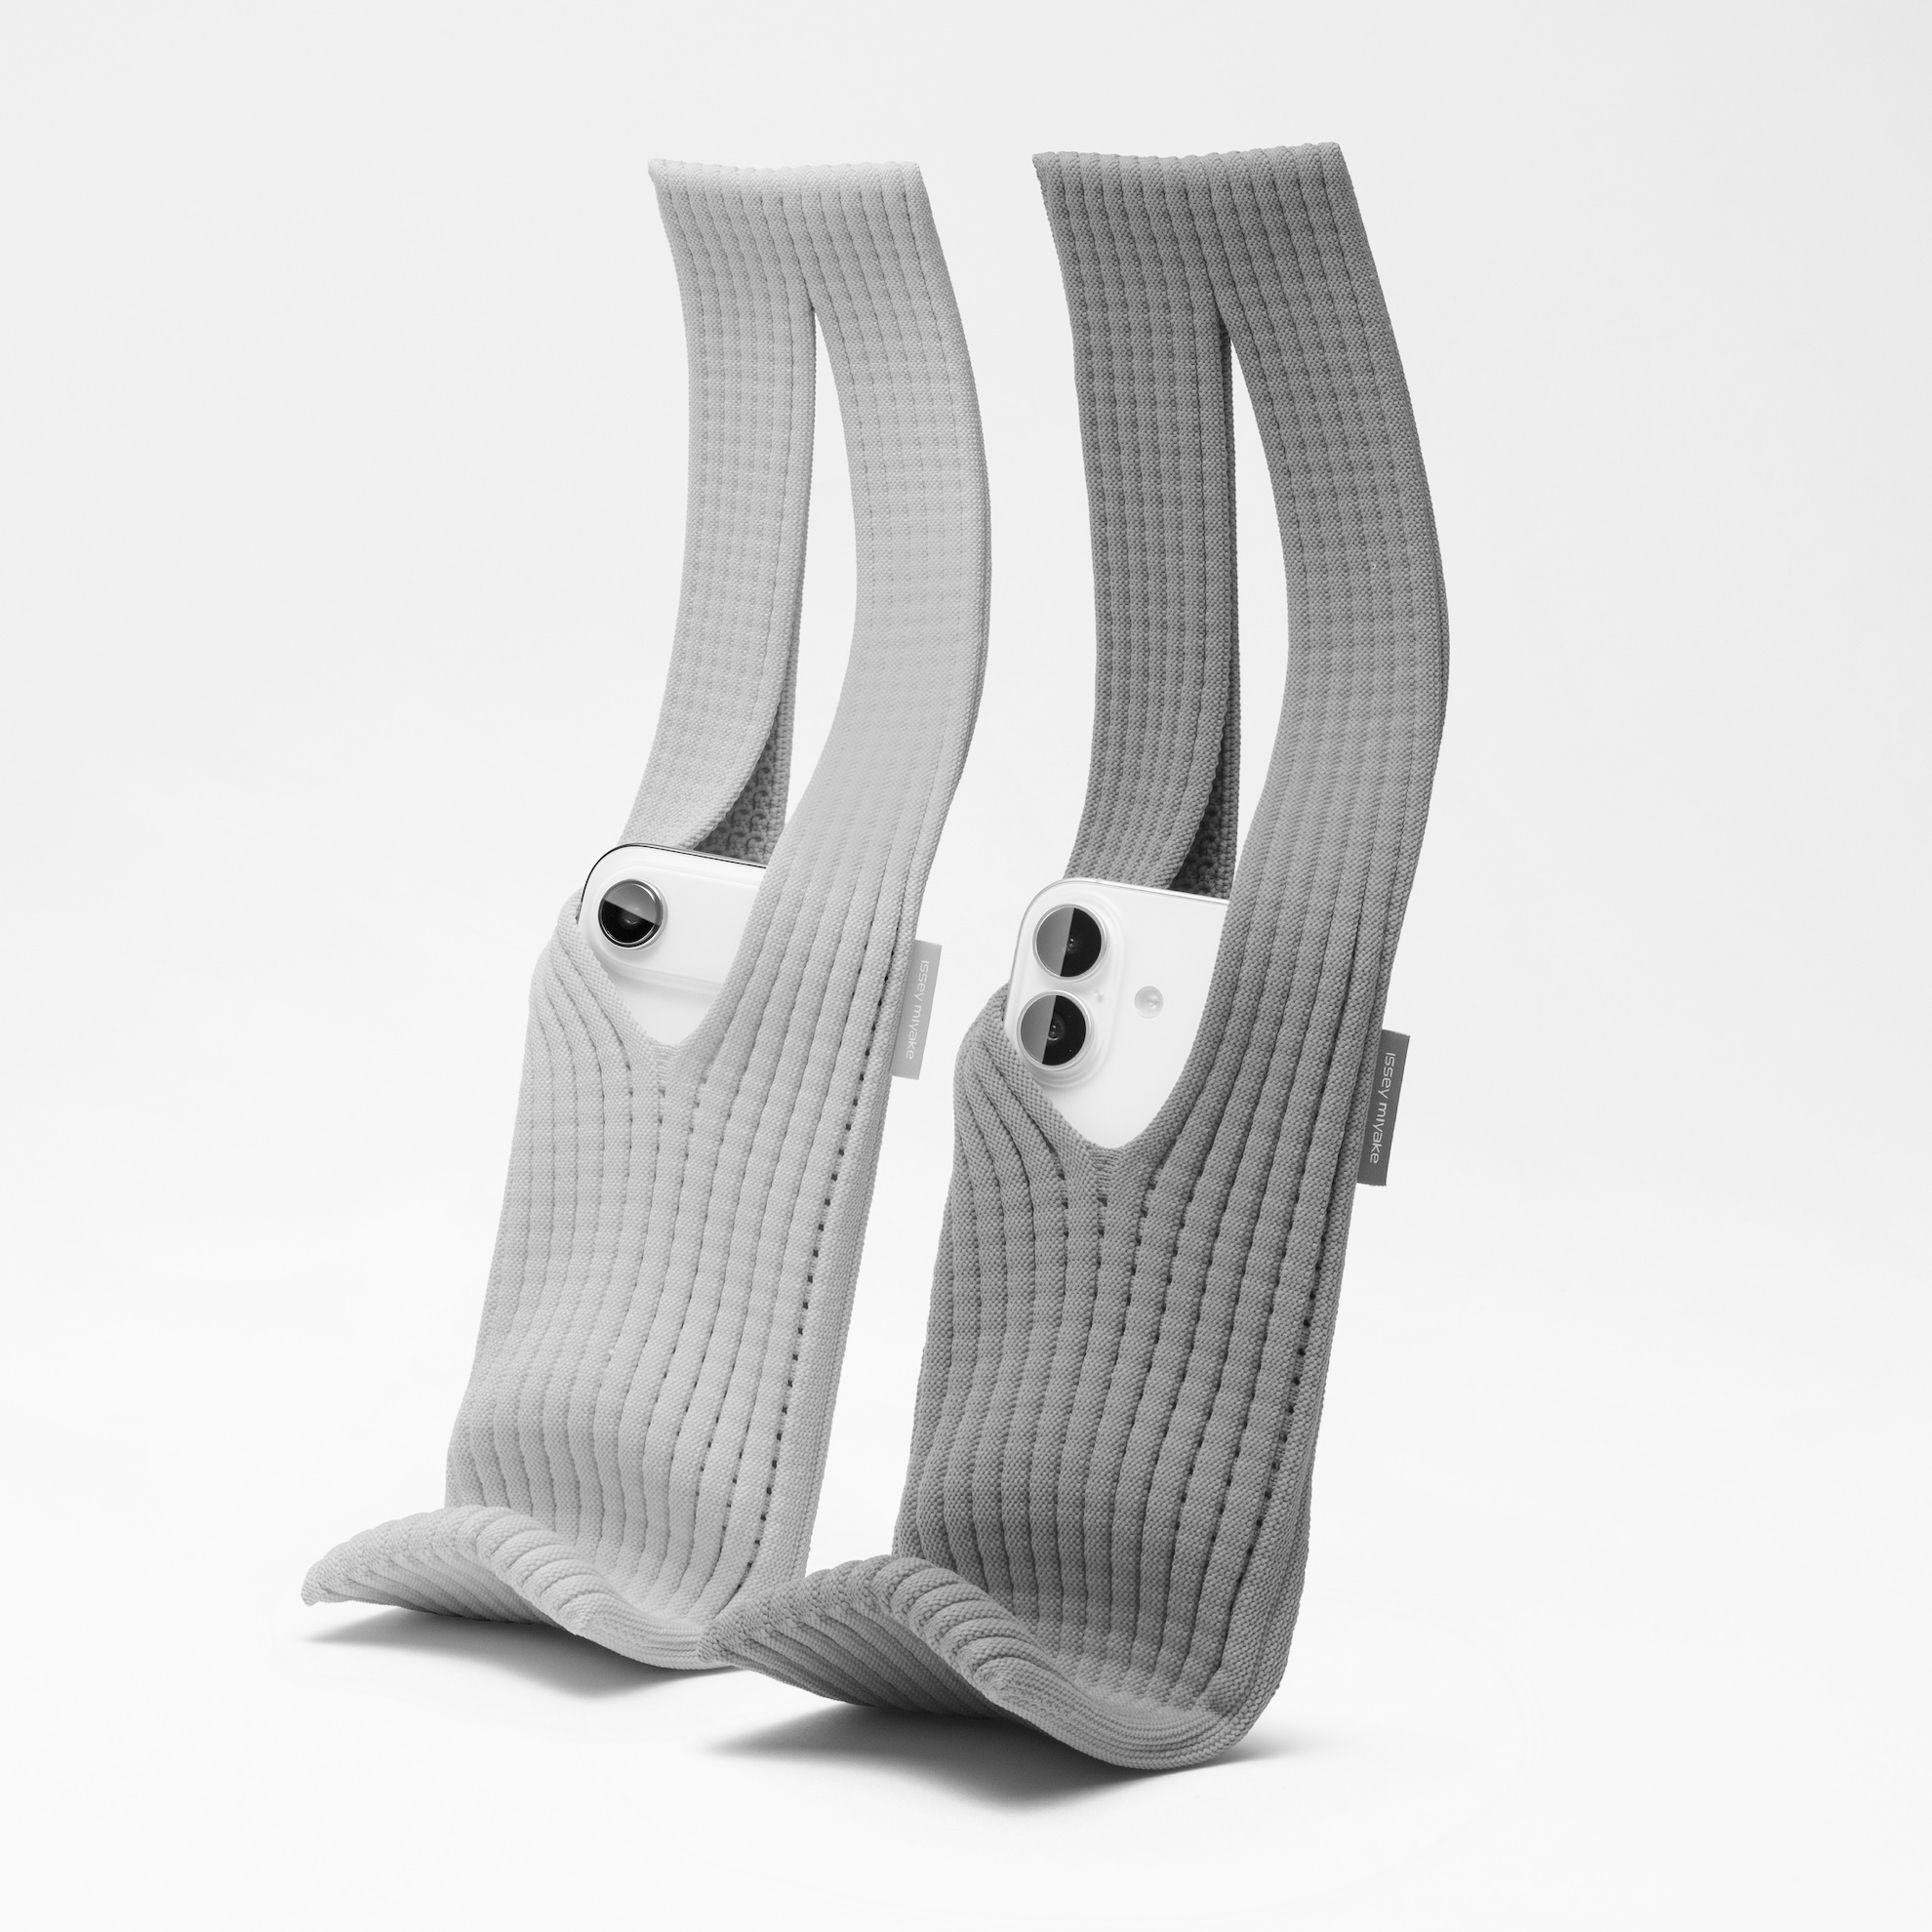
\includegraphics[width=0.45\textwidth]{zad2/oryginal.png}
\caption{Obraz oryginalny.}
\end{figure}

\begin{figure}[H]
\centering
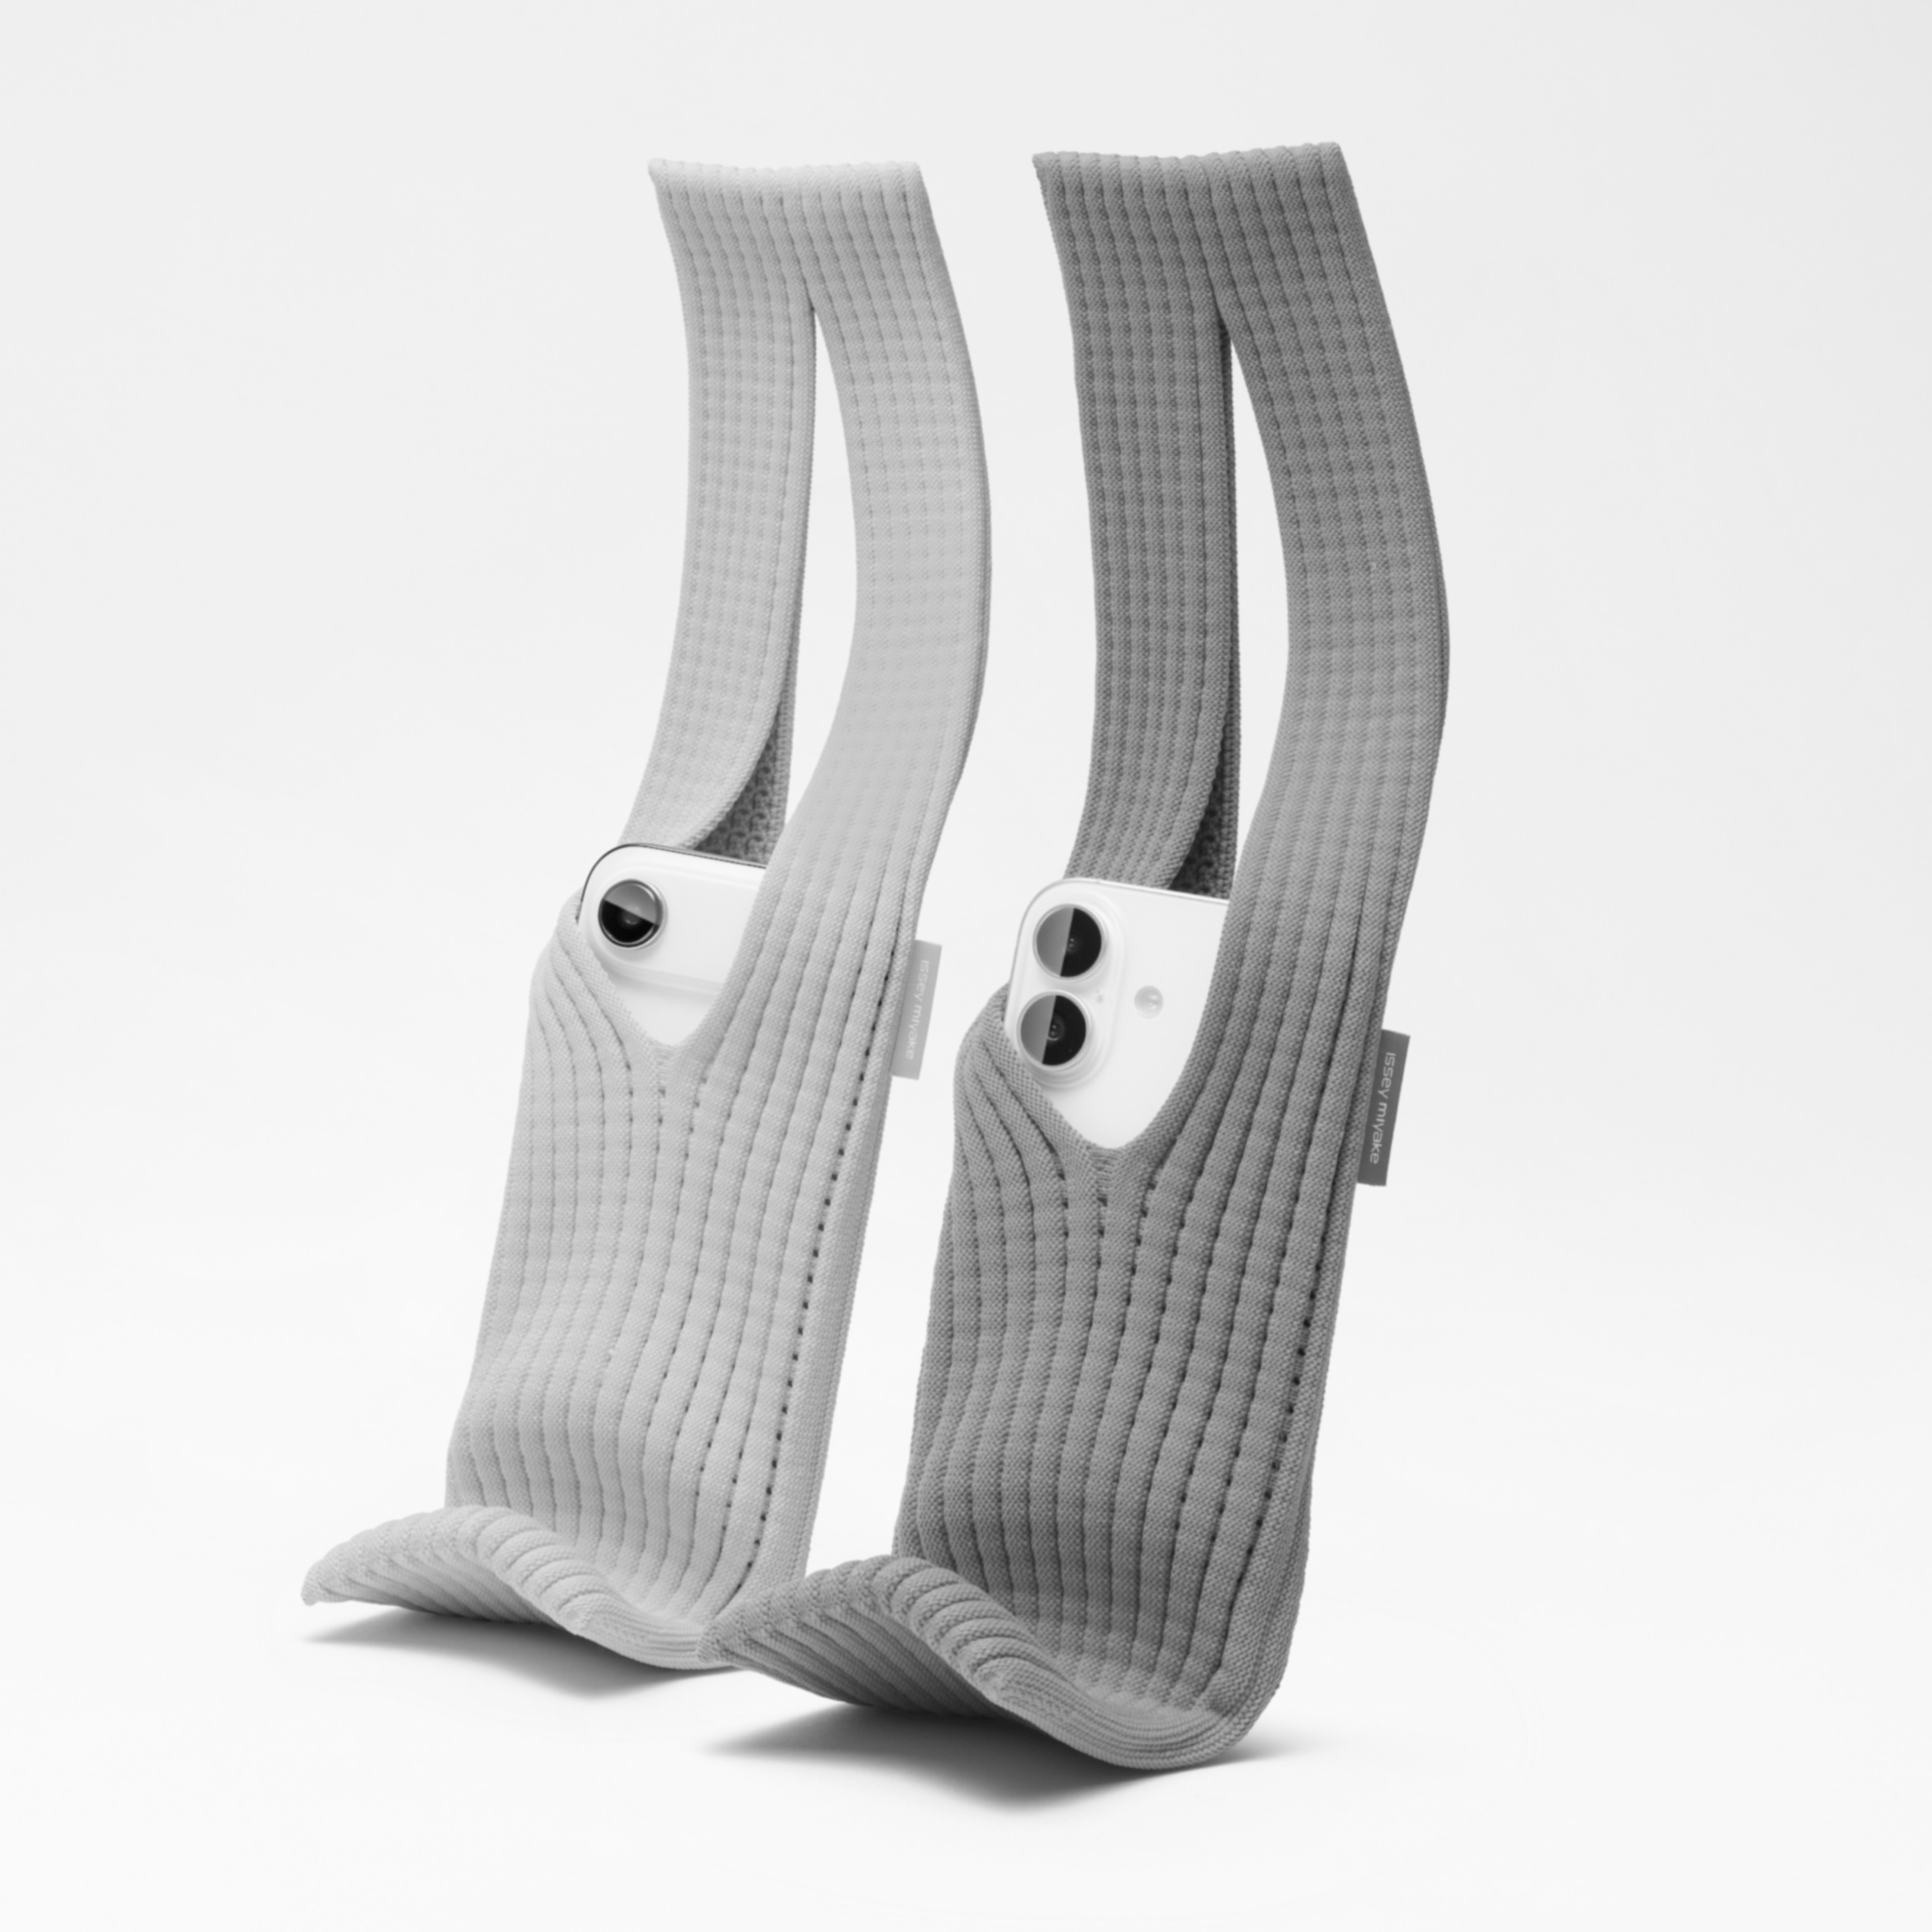
\includegraphics[width=0.45\textwidth]{zad2/h_a.png}
\caption{Wynik filtracji jądrem $h_a$}
\end{figure}

\begin{figure}[H]
\centering
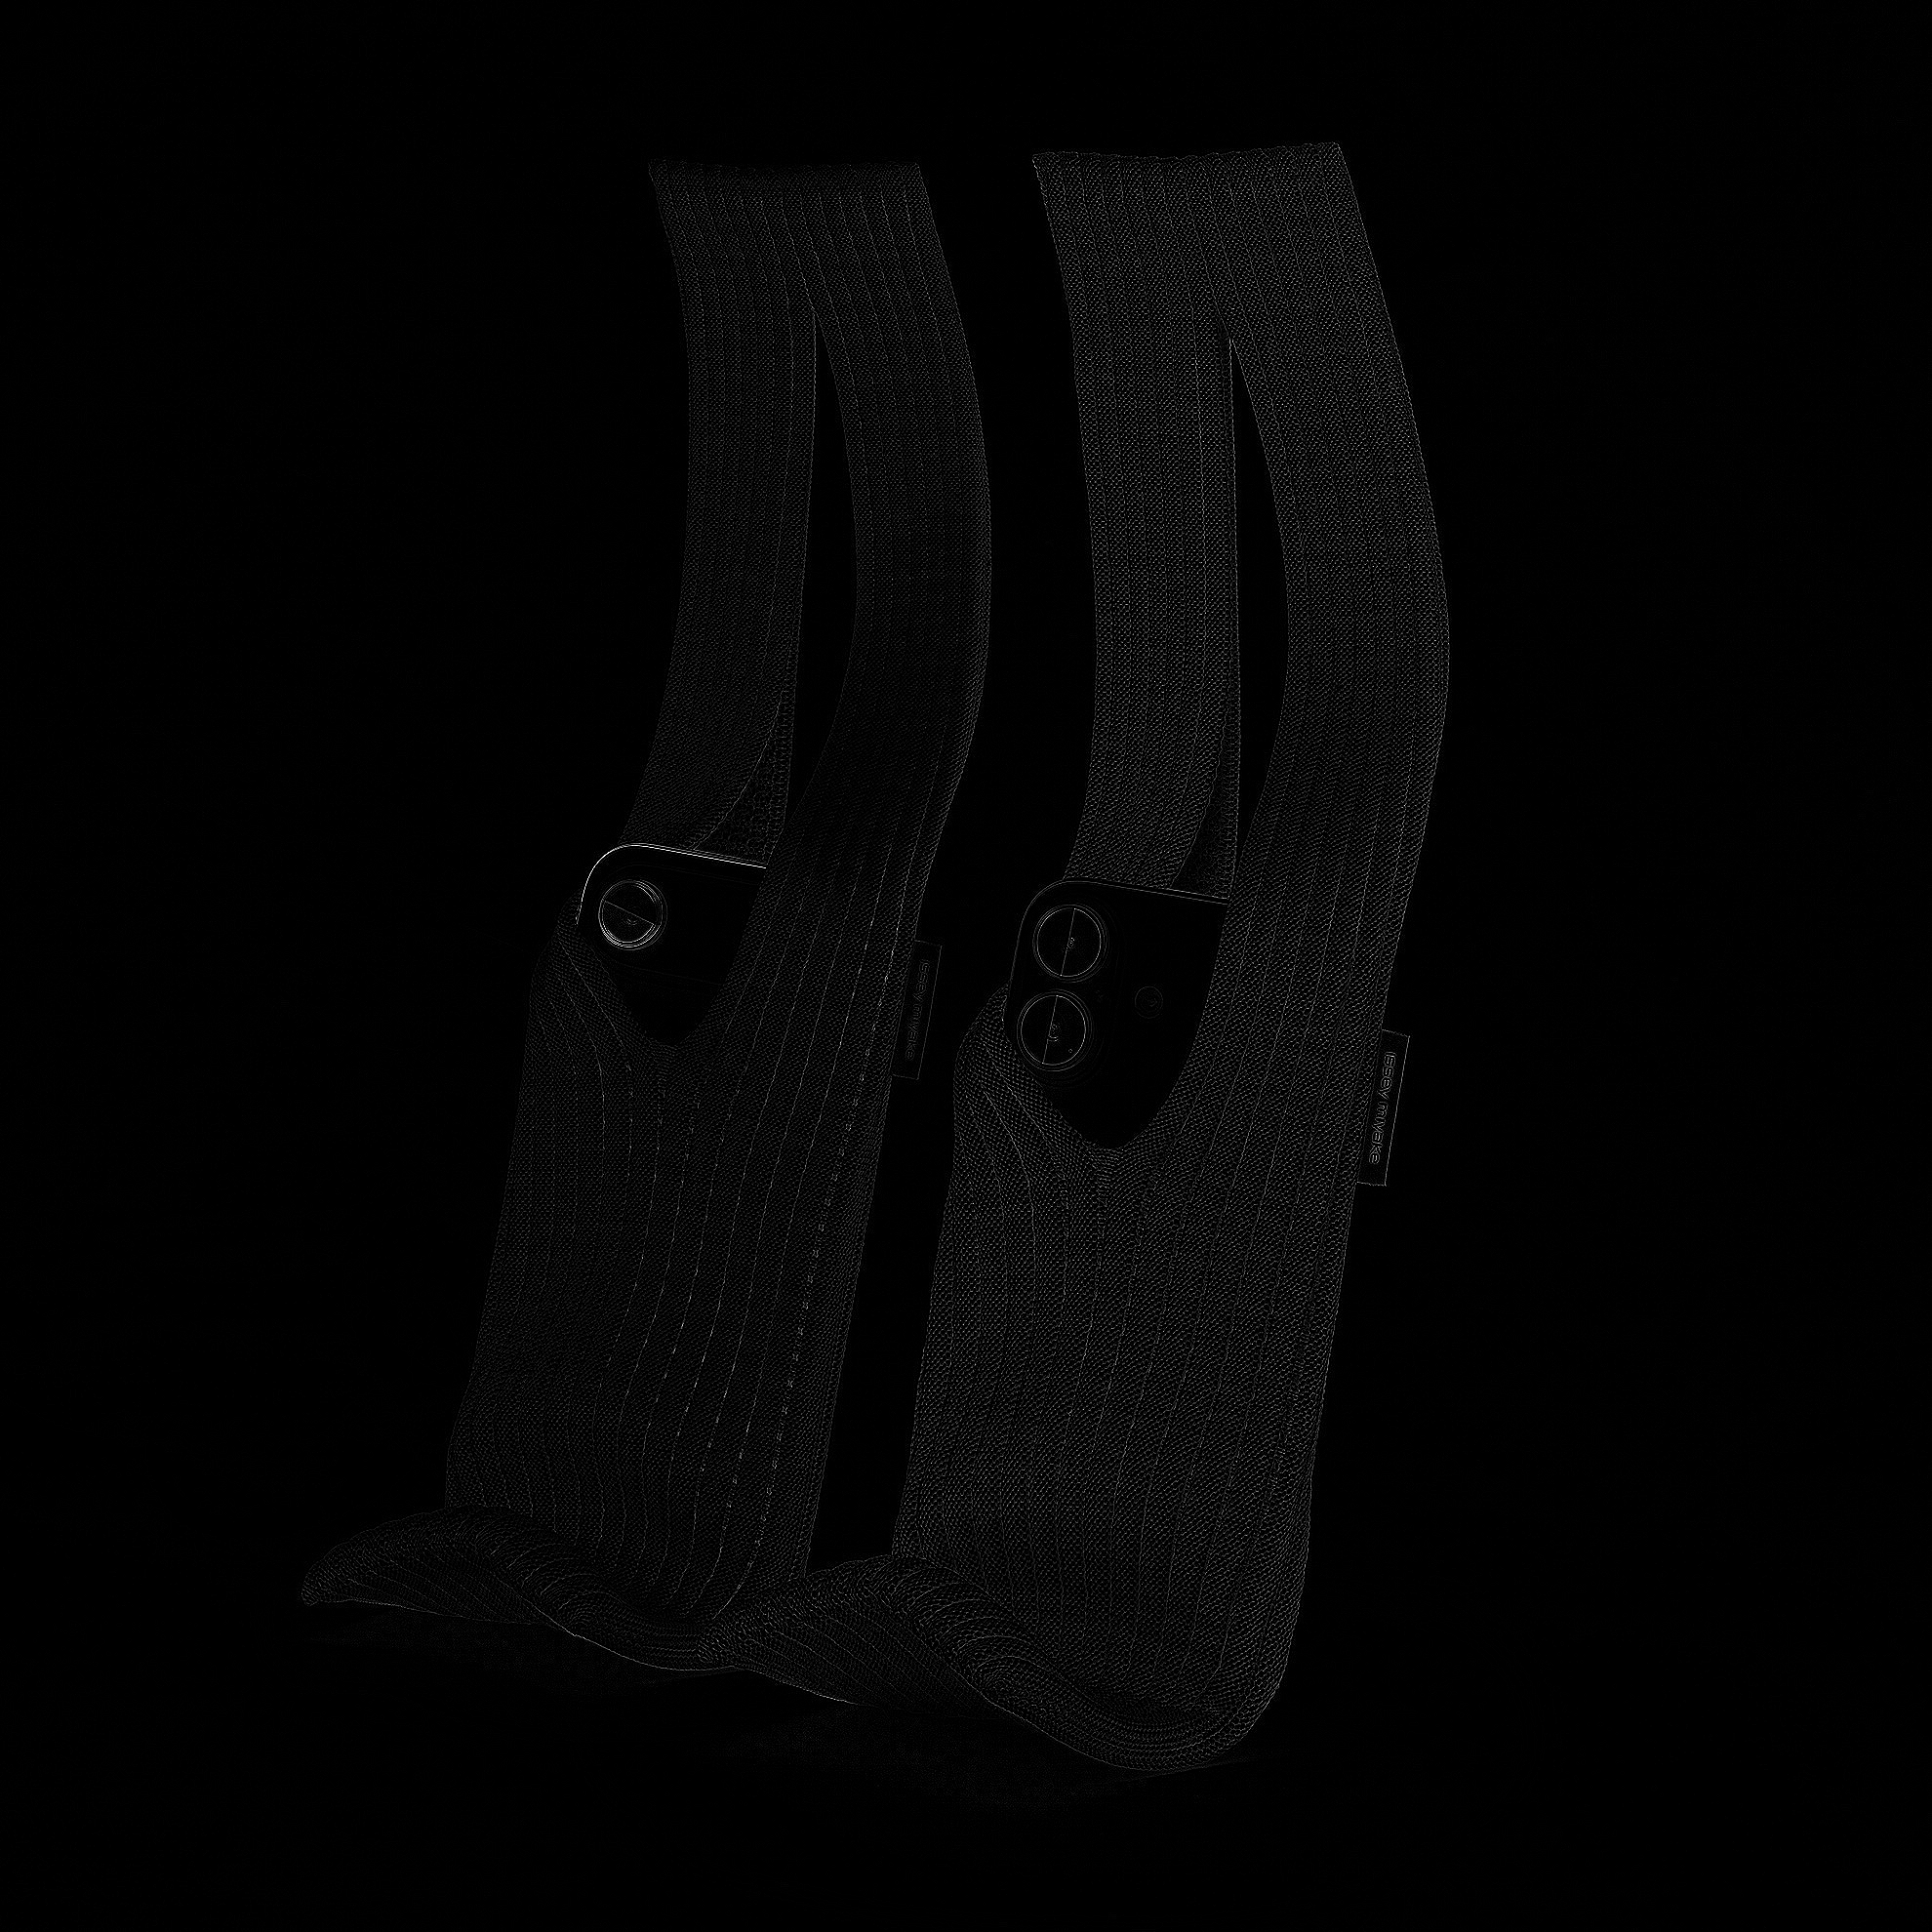
\includegraphics[width=0.45\textwidth]{zad2/h_b.png}
\caption{Wynik filtracji jądrem $h_b$}
\end{figure}

\begin{figure}[H]
\centering
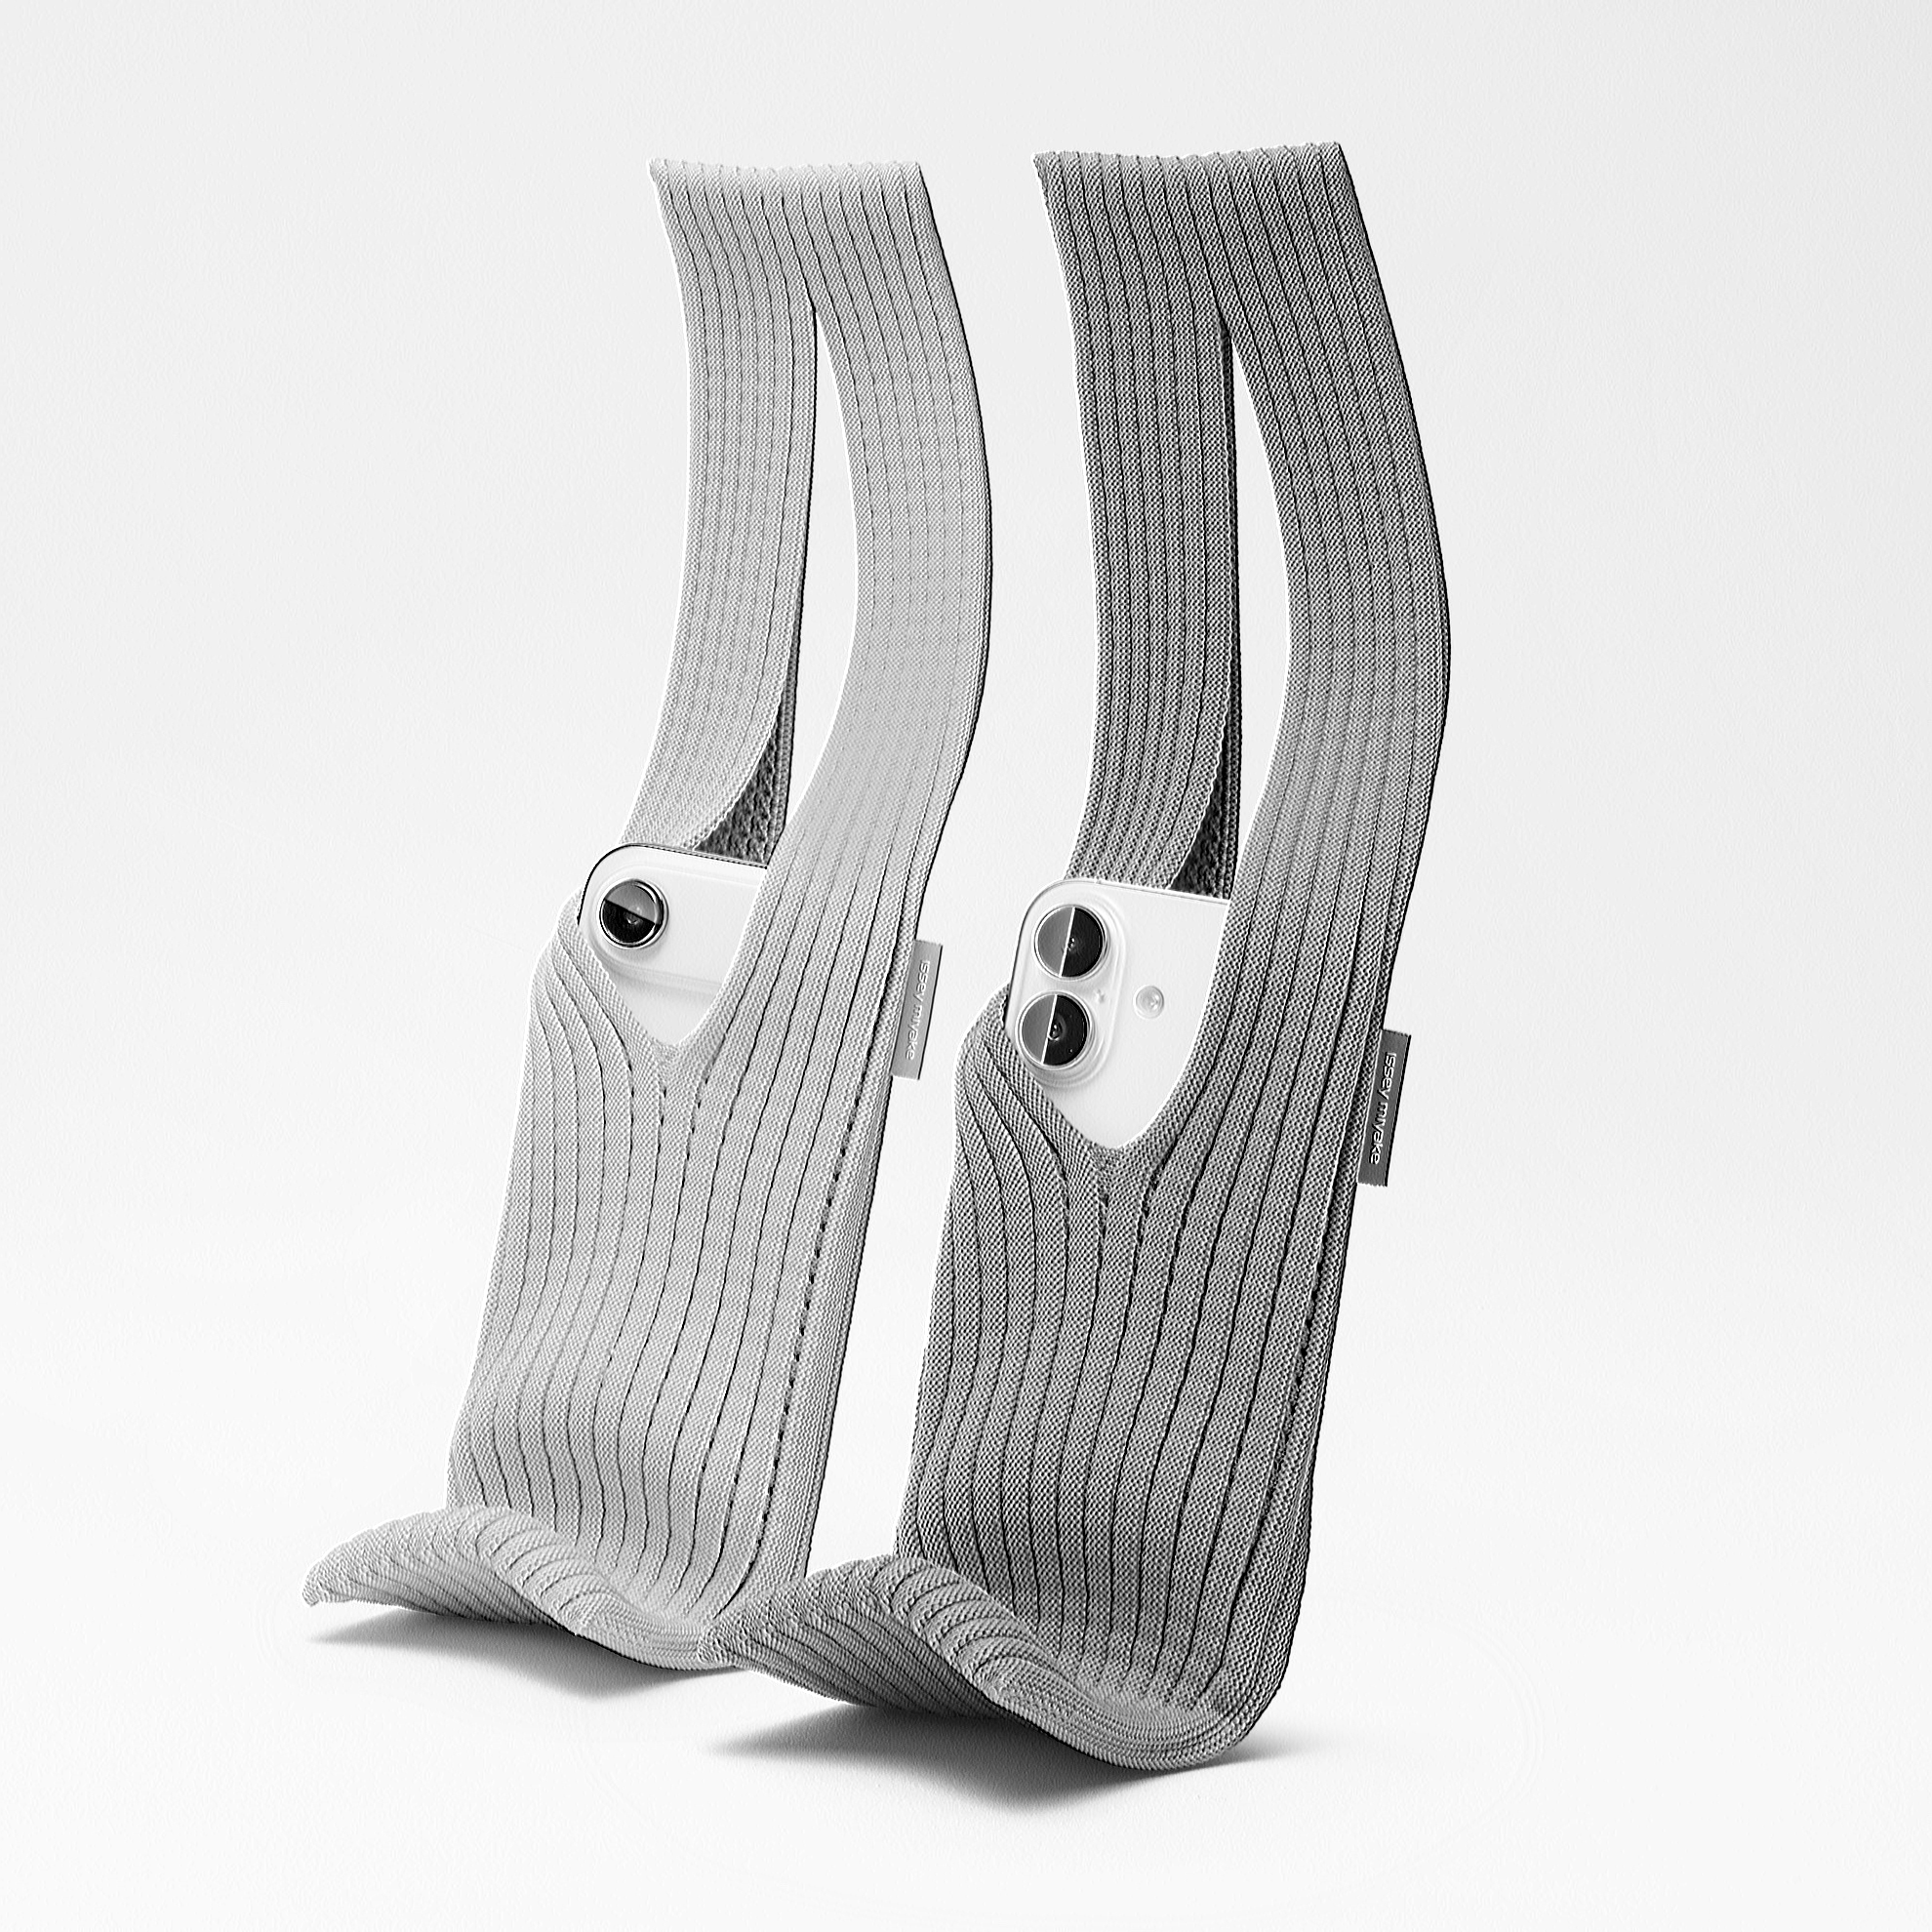
\includegraphics[width=0.45\textwidth]{zad2/h_c.png}
\caption{Wynik filtracji jądrem $h_c$}
\end{figure}

\begin{figure}[H]
\centering
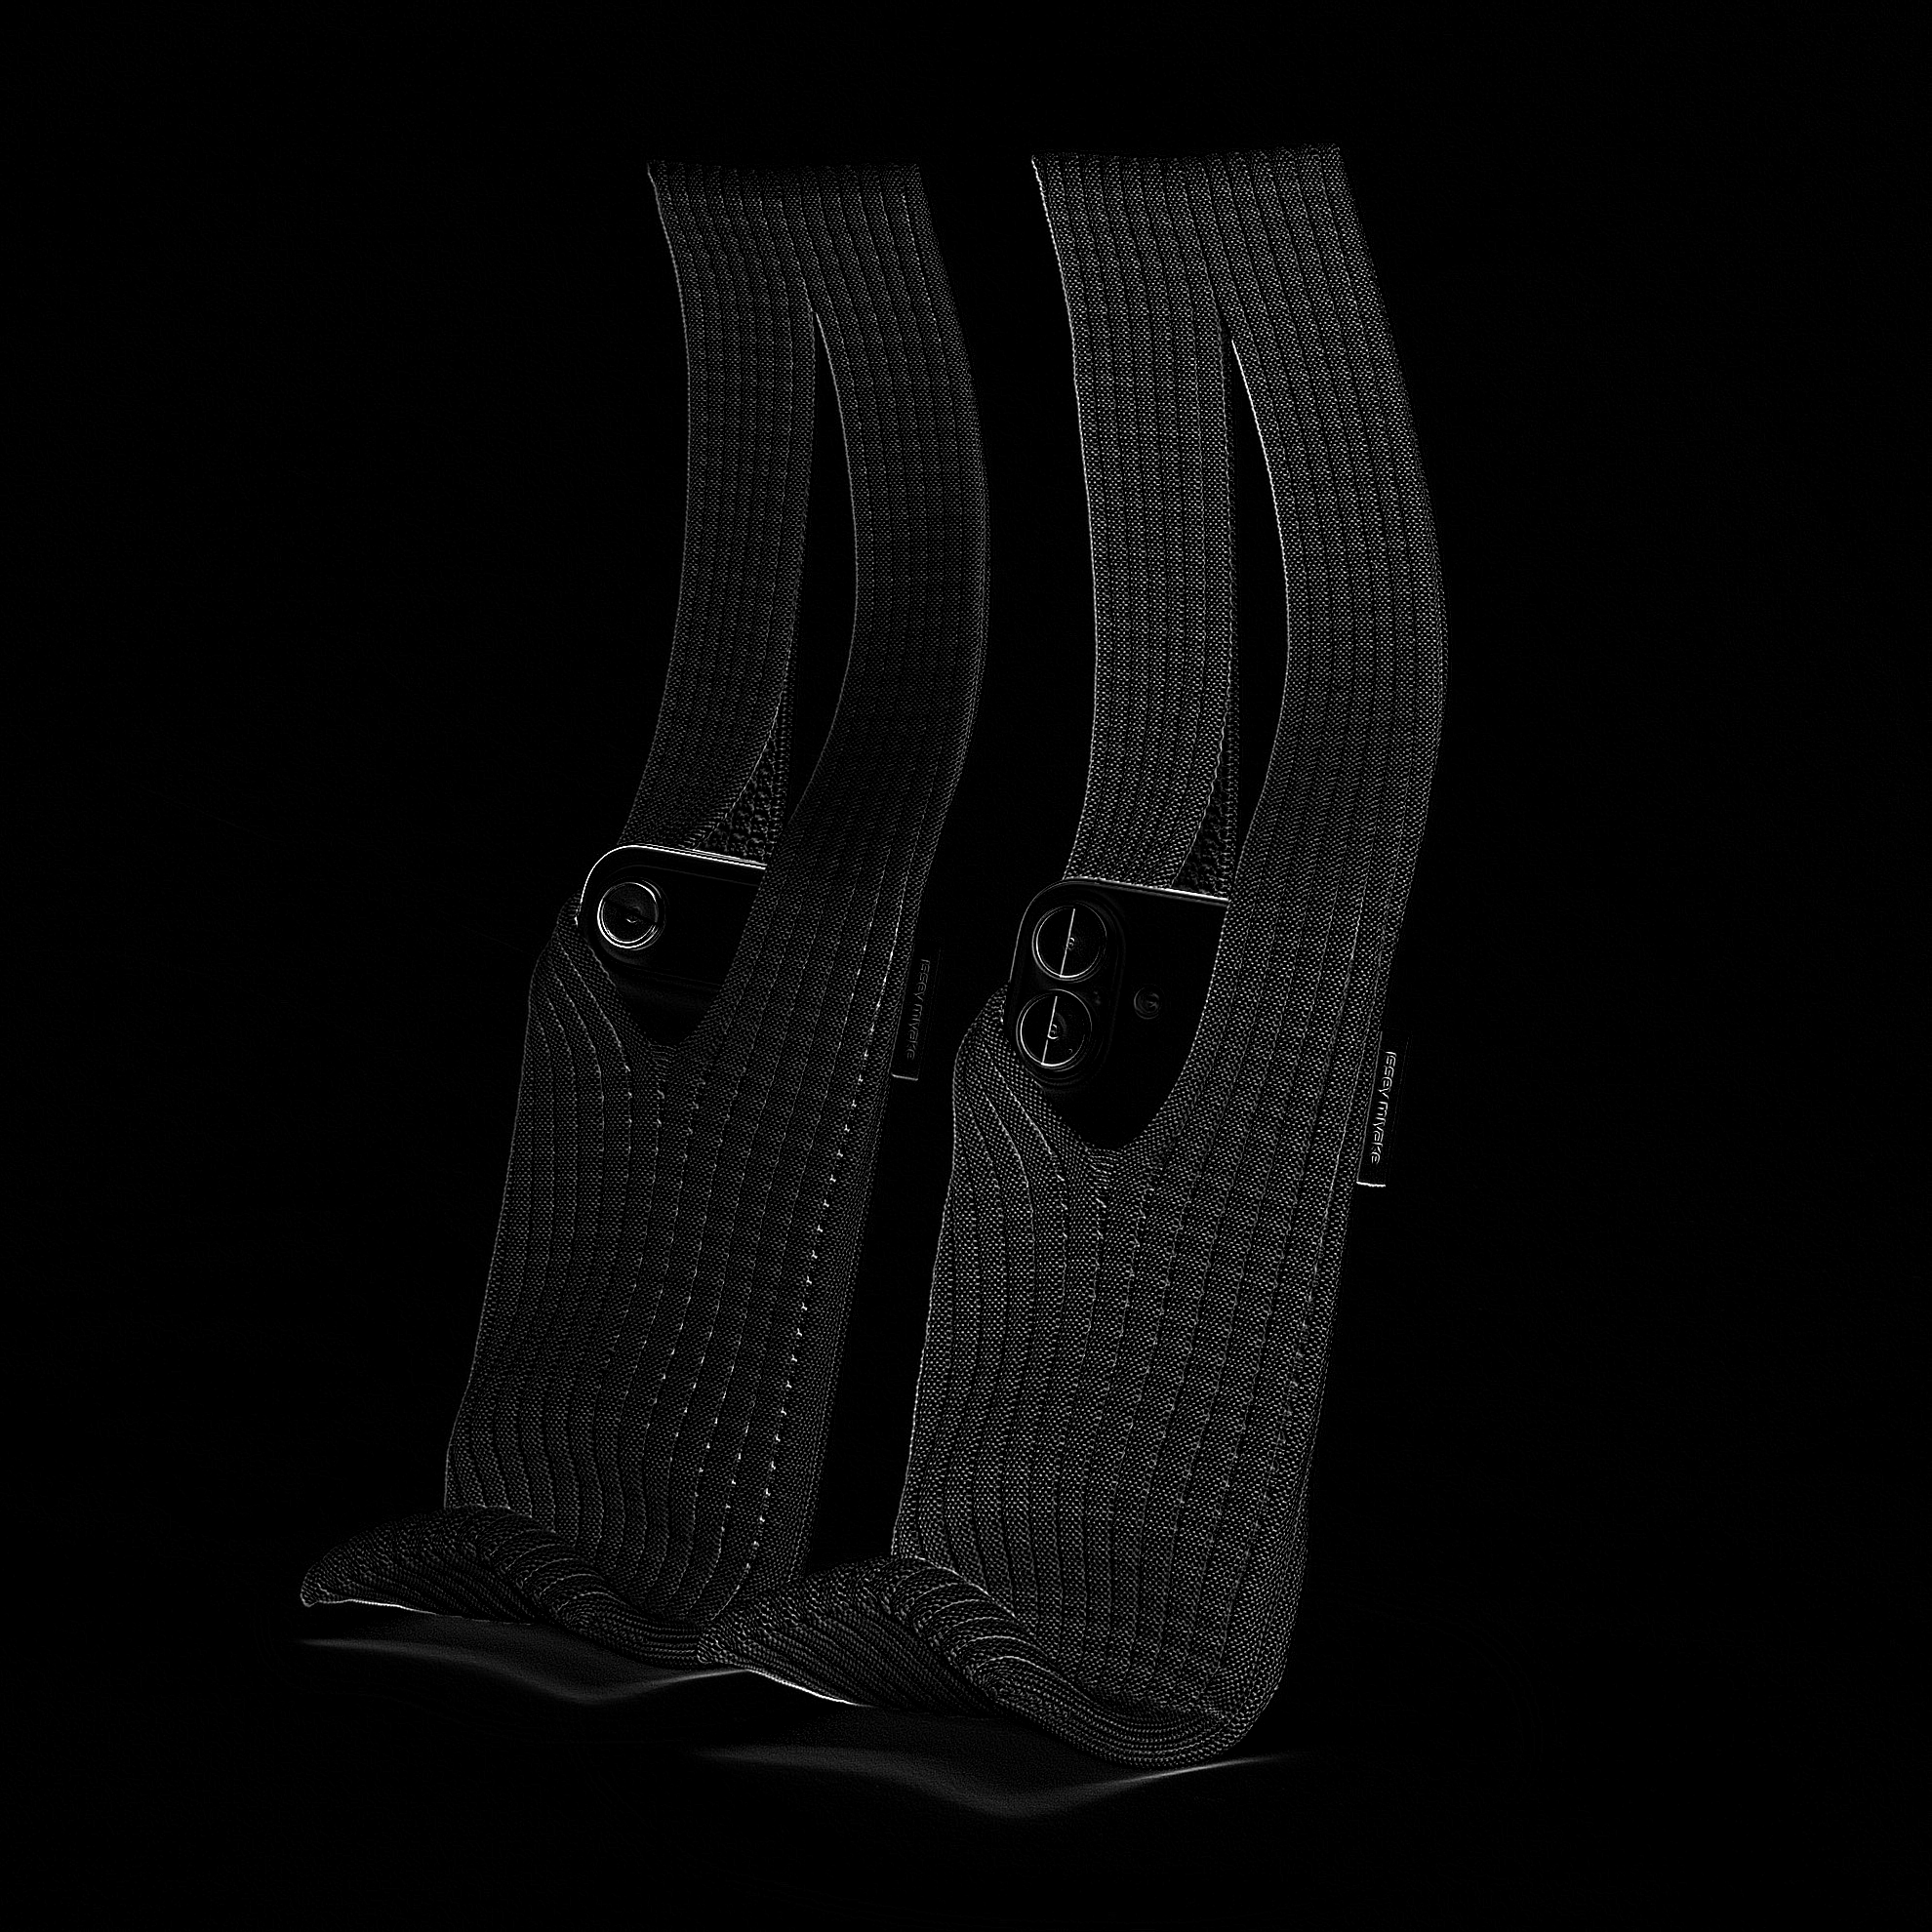
\includegraphics[width=0.45\textwidth]{zad2/h_d.png}
\caption{Wynik filtracji jądrem $h_d$}
\end{figure}

\subsection*{(b) Charakterystyka filtrów}

\textbf{Filtry dolnoprzepustowe:} jądro $h_a$ \newline
\textbf{Filtry górnoprzepustowe:} jądra $h_b$, $h_c$, $h_d$ \newline
\textbf{Filtr $h_c$:} Filtr ten uwypukla przede wszystkim krawędzie pionowe. \newline
\textbf{Filtr $h_d$:} Jest to filtr kierunkowy, który najlepiej wykrywa krawędzie przebiegające pod kątem (skosie).

\section*{Zadanie 3 - Splot jąder filtrów}

\subsection*{(a) Obrazy $g_1 = g * h_1$ oraz $g_2 = g_1 * h_2$}

\begin{figure}[H]
\centering

\includegraphics[width=0.45\textwidth]{zad3/oryginal.png}
\caption{Obraz oryginalny $g$.}
\end{figure}

\begin{figure}[H]
\centering
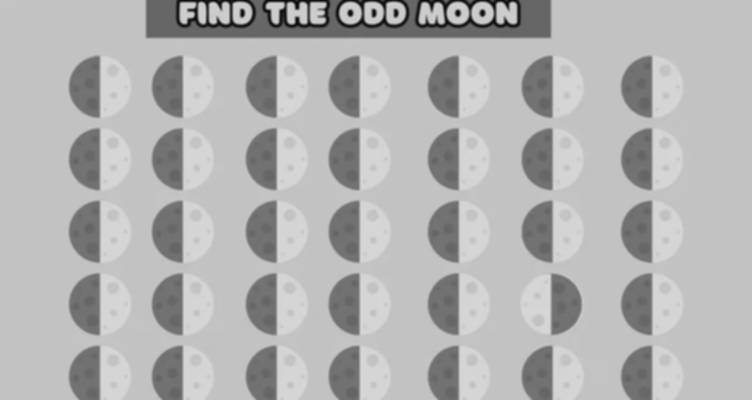
\includegraphics[width=0.45\textwidth]{zad3/g1.png}
\caption{$g_1 = g * h_1$}
\end{figure}

\begin{figure}[H]
\centering
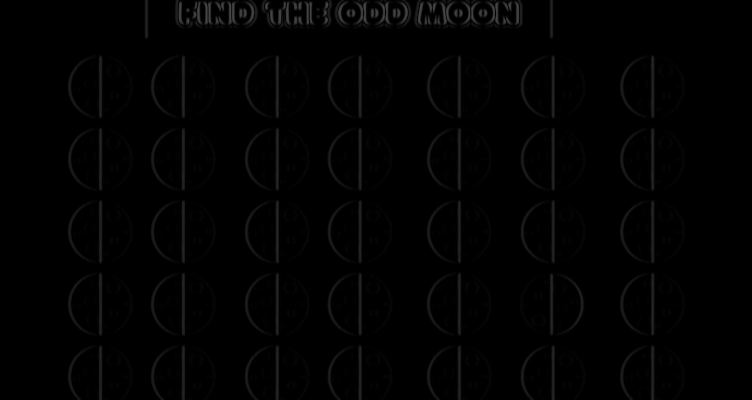
\includegraphics[width=0.45\textwidth]{zad3/g2.png}
\caption{$g_2 = g_1 * h_2$}
\end{figure}

\subsection*{(b) Złożone jądro $h_3 = h_1 * h_2$ oraz $g_3 = g * h_3$}

\begin{figure}[H]
\centering
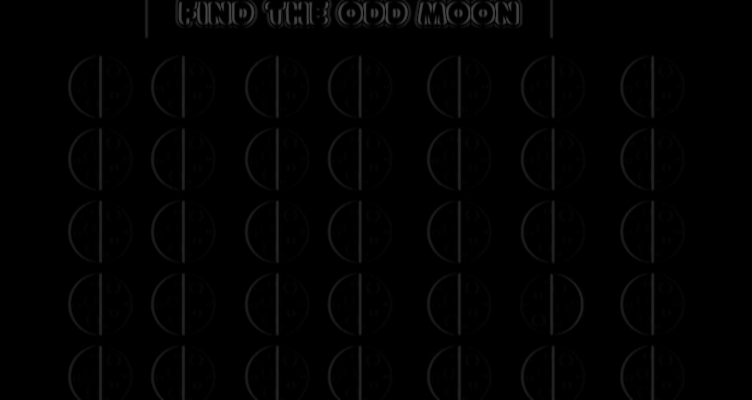
\includegraphics[width=0.45\textwidth]{zad3/g3.png}
\caption{$g_3 = g * h_3$ - wynik filtracji obrazu oryginalnego złożonym jądrem $h_3$.}
\end{figure}

\begin{figure}[H]
\centering
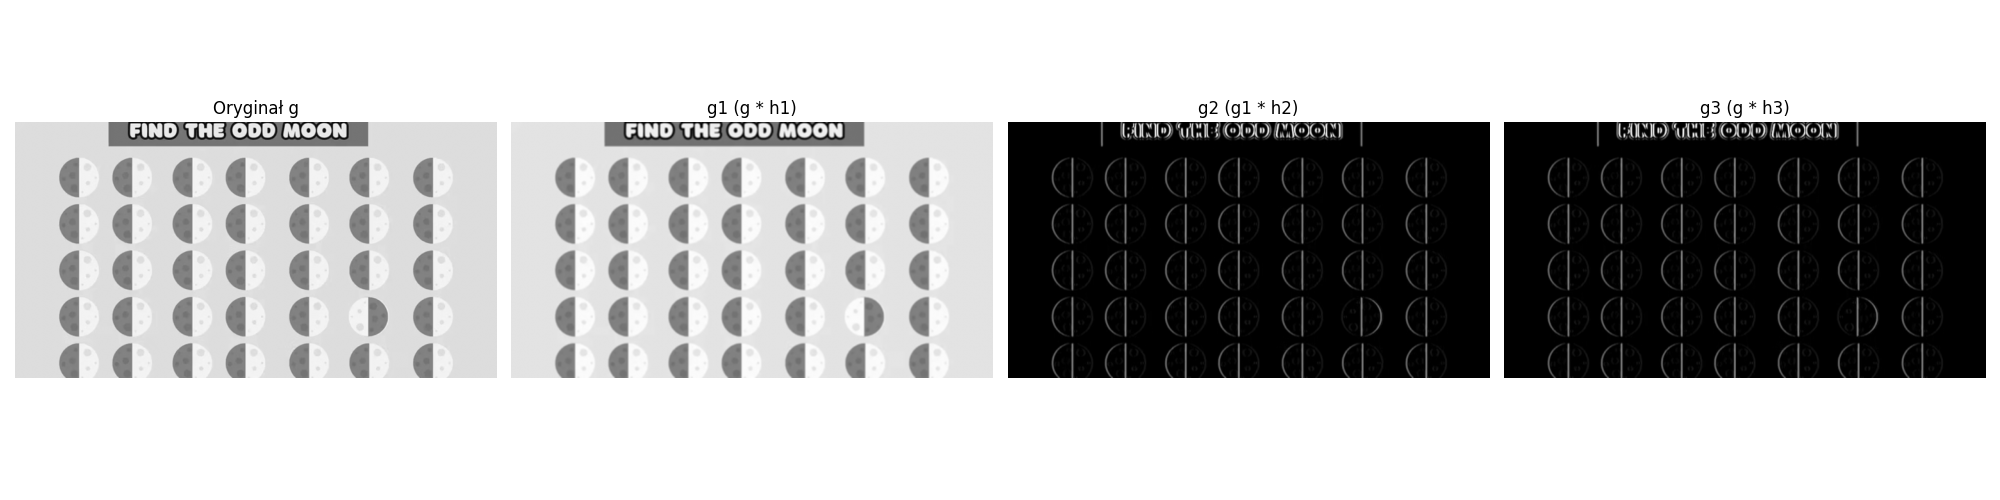
\includegraphics[width=\textwidth]{zad3/zestawienie_splotu.png}
\caption{Zestawienie}
\end{figure}

\subsection*{(c) Interpretacja}

Maksymalna różnica między obrazami $g_2$ a $g_3$ wynosi blisko zeru (różnica wynika wyłącznie z błędów numerycznych zmiennoprzecinkowych). Obrazy $g_2$ i $g_3$ są więc praktycznie identyczne.

\section*{Zadanie 4 - Znajdywanie krawędzi w obrazie}

\subsection*{(a) Pochodne $g_1 = g * h_1$ oraz $g_2 = g * h_2$}

\begin{figure}[H]
\centering

\includegraphics[width=0.45\textwidth]{zad4/oryginal.png}
\caption{Obraz oryginalny $g$.}
\end{figure}

\begin{figure}[H]
\centering

\includegraphics[width=0.45\textwidth]{zad4/g1.png}
\caption{$g_1 = g * h_1$ - pochodna pionowa.}
\end{figure}

\begin{figure}[H]
\centering

\includegraphics[width=0.45\textwidth]{zad4/g2.png}
\caption{$g_2 = g * h_2$ - pochodna pozioma.}
\end{figure}

\subsection*{(b) Obraz wyjściowy $g_3$}

\begin{figure}[H]
\centering

\includegraphics[width=0.45\textwidth]{zad4/g3.png}
\caption{$g_3 = \sqrt{g_1^2 + g_2^2}$}
\end{figure}

\begin{figure}[H]
\centering
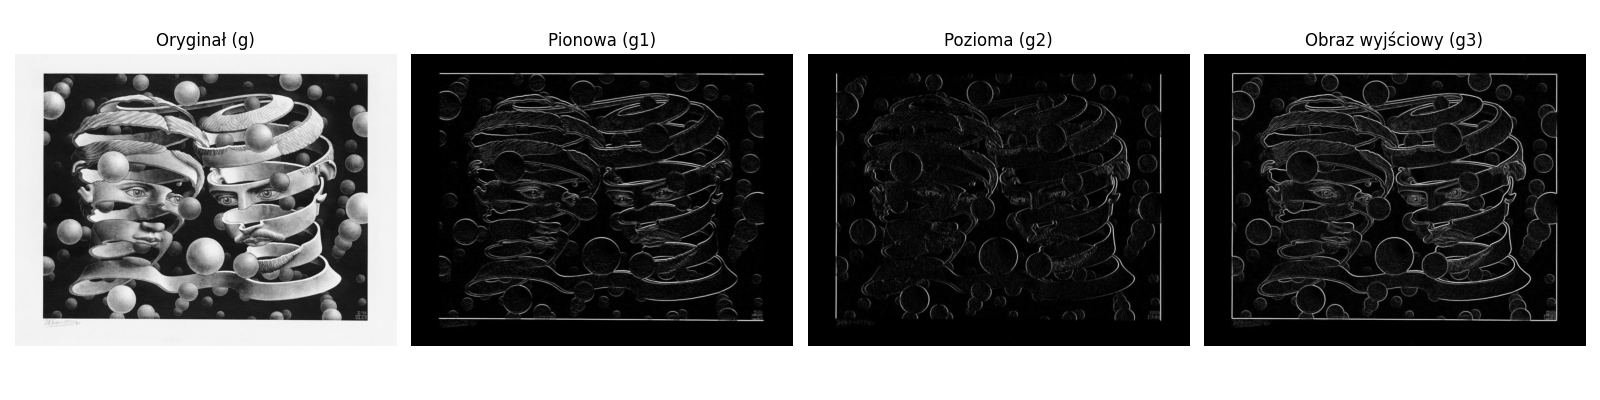
\includegraphics[width=\textwidth]{zad4/zestawienie_sobel.png}
\caption{Zestawienie: oryginał, pochodna pionowa $g_1$, pochodna pozioma $g_2$, obraz wyjściowy $g_3$.}
\end{figure}

\subsection*{(c) Porównanie z funkcją Find Edges w ImageJ}

\begin{figure}[H]
\centering
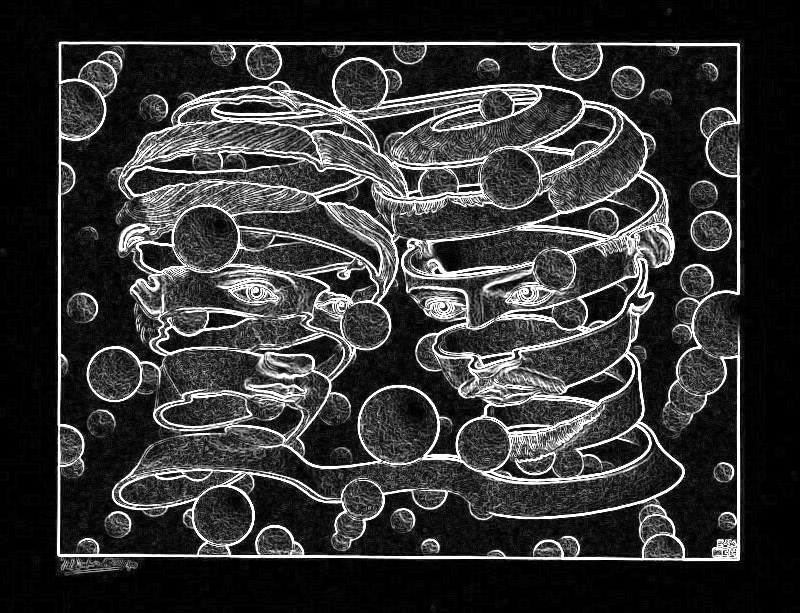
\includegraphics[width=0.45\textwidth]{zad4/imageJEscher.png}
\caption{Wynik funkcji \texttt{Find Edges} w ImageJ.}
\end{figure}

Wynik własnej implementacji $g_3$ jest wizualnie i ilościowo bardzo zbliżony do wyniku zwracanego przez funkcję \texttt{Find Edges} z ImageJ. Wynika to z faktu, że ImageJ realizuje dokładnie tę samą operację:
\begin{itemize}
    \item splot obrazu z dwoma operatorami Sobela $h_1$ (pionowy) oraz $h_2$ (poziomy),
    \item złożenie pochodnych w obrazie wyjściowym $\sqrt{g_1^2 + g_2^2}$.
\end{itemize}

\section*{Zadanie 5 -- Detektor krawędzi Kirscha}

\subsection*{(a) Krawędzie obrazu wyznaczone detektorem Kirscha}

\begin{figure}[H]
\centering
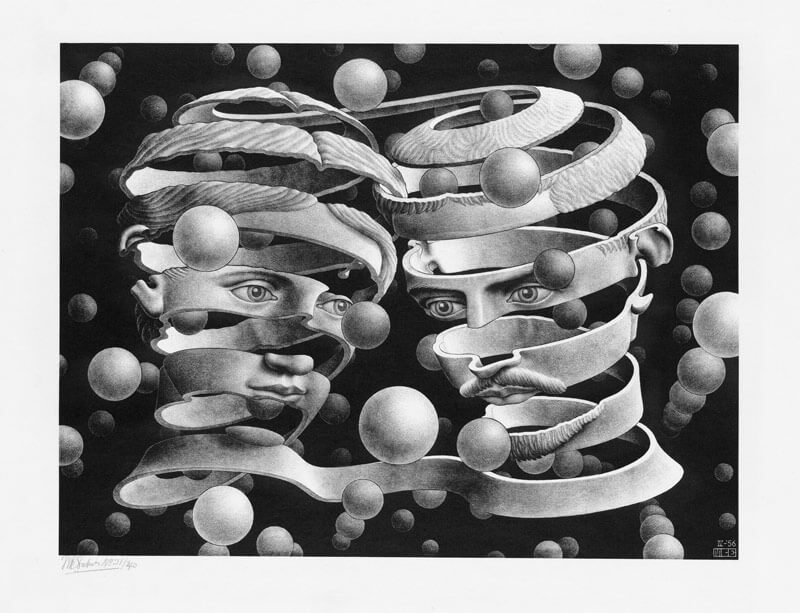
\includegraphics[width=0.45\textwidth]{zad5/Escher.png}
\caption{Obraz oryginalny $g$.}
\end{figure}

\begin{figure}[H]
\centering
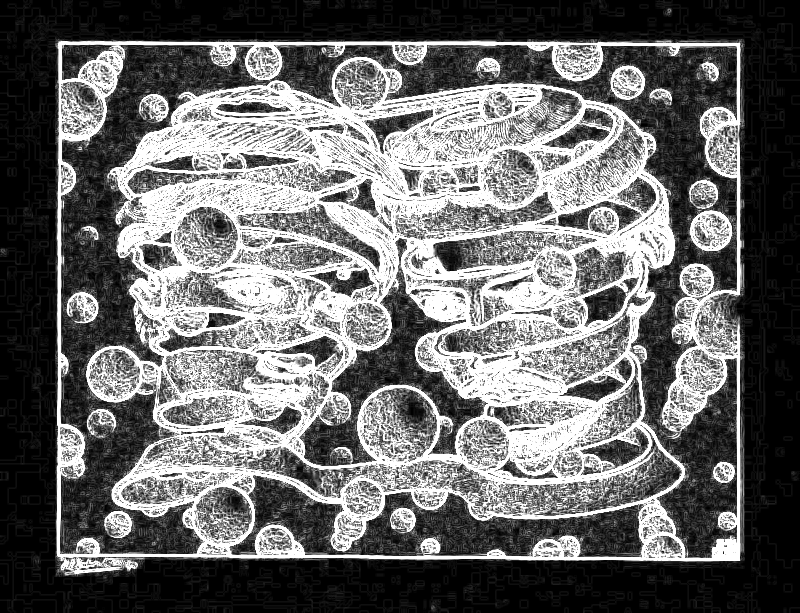
\includegraphics[width=0.45\textwidth]{zad5/krawedzie_kirscha.png}
\caption{Krawędzie wyznaczone detektorem Kirscha.}
\end{figure}

\subsection*{(b) Porównanie z funkcją Find Edges w ImageJ}

\begin{figure}[H]
\centering
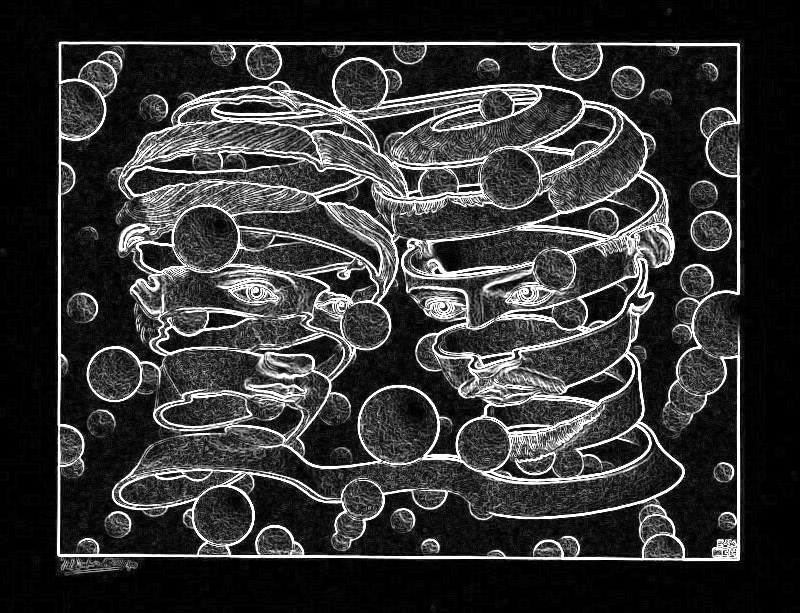
\includegraphics[width=0.45\textwidth]{zad4/imageJEscher.png}
\caption{Wynik funkcji \texttt{Find Edges} w ImageJ (operator Sobela).}
\end{figure}

Detektor Kirscha i \texttt{Find Edges} (Sobel) z ImageJ dają zbliżone mapy krawędzi. Oba detektory rozwiązują ten sam problem (lokalna detekcja gradientu), ale Kirsch jest bardziej kierunkowy i bardziej czuły, kosztem większej podatności na szum i szybszego nasycenia w 8-bitowej reprezentacji.

\section*{Zadanie 6 -- Highboost filtering}

\subsection*{Wyniki}

\begin{figure}[H]
\centering

\includegraphics[width=0.45\textwidth]{zad6/oryginal.png}
\caption{Obraz oryginalny $g$.}
\end{figure}

\begin{figure}[H]
\centering
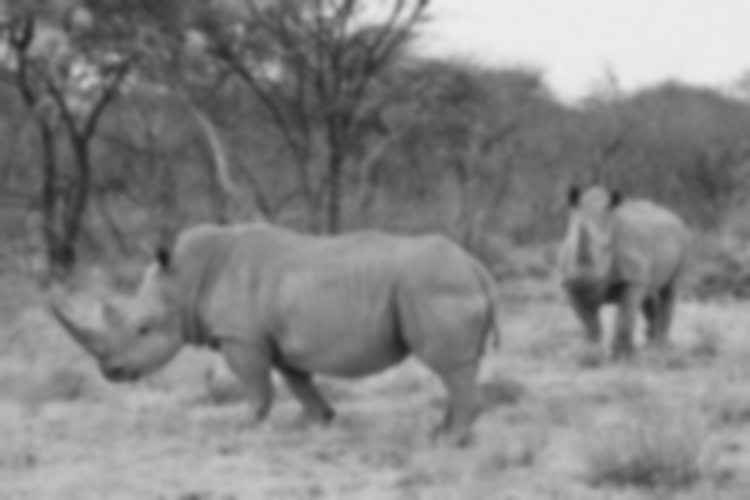
\includegraphics[width=0.45\textwidth]{zad6/blurred.png}
\caption{Obraz po wygładzeniu filtrem Gaussa $g_b$.}
\end{figure}

\begin{figure}[H]
\centering
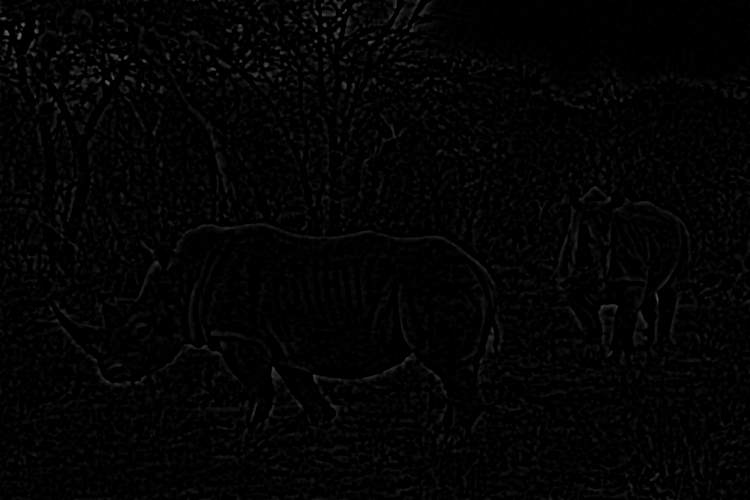
\includegraphics[width=0.45\textwidth]{zad6/unsharp_mask_view.png}
\caption{Nieostra maska $m = g - g_b$ -- zawiera krawędzie i detale wysokoczęstotliwościowe.}
\end{figure}

\begin{figure}[H]
\centering
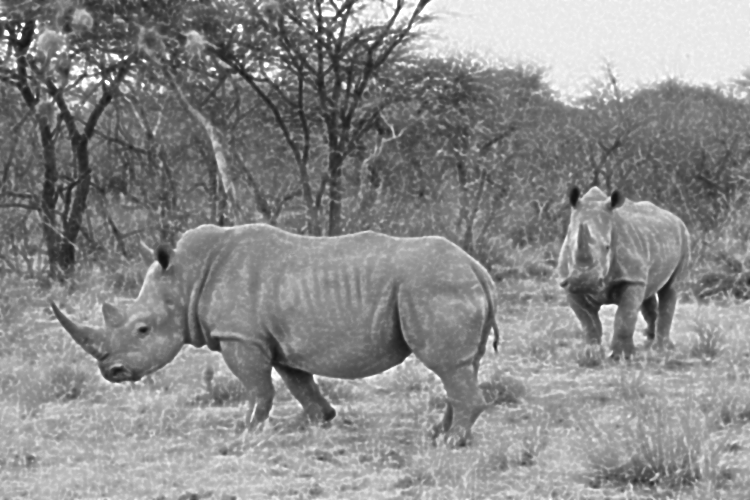
\includegraphics[width=0.45\textwidth]{zad6/highboost.png}
\caption{Wynik highboost filtering: $g_{\mathrm{HB}} = g + k\cdot m$ dla $k=1{,}5$.}
\end{figure}

\begin{figure}[H]
\centering
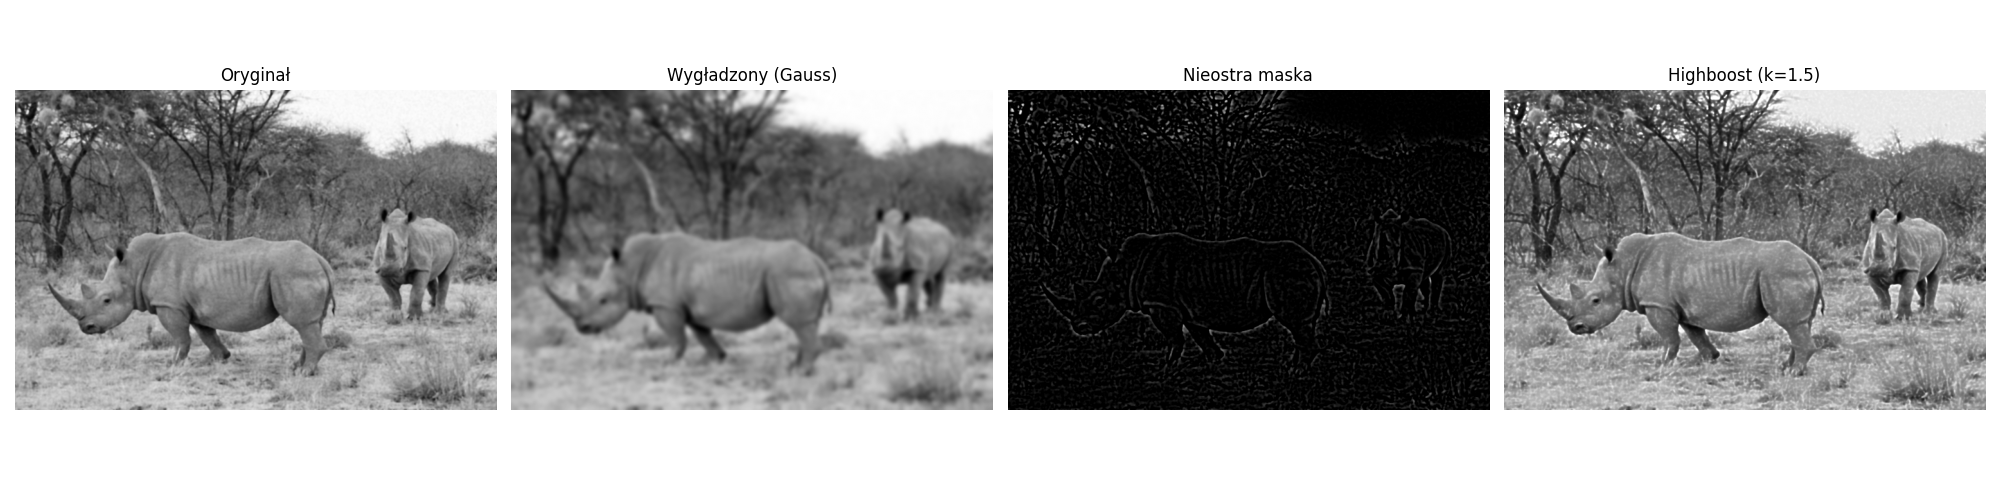
\includegraphics[width=\textwidth]{zad6/highboost_result.png}
\caption{Zestawienie: oryginał, wygładzenie Gaussa, nieostra maska, wynik highboost.}
\end{figure}

\section*{Zadanie 7 -- Dekonwolucja obrazu}

\subsection*{Obraz wejściowy}

\begin{figure}[H]
\centering
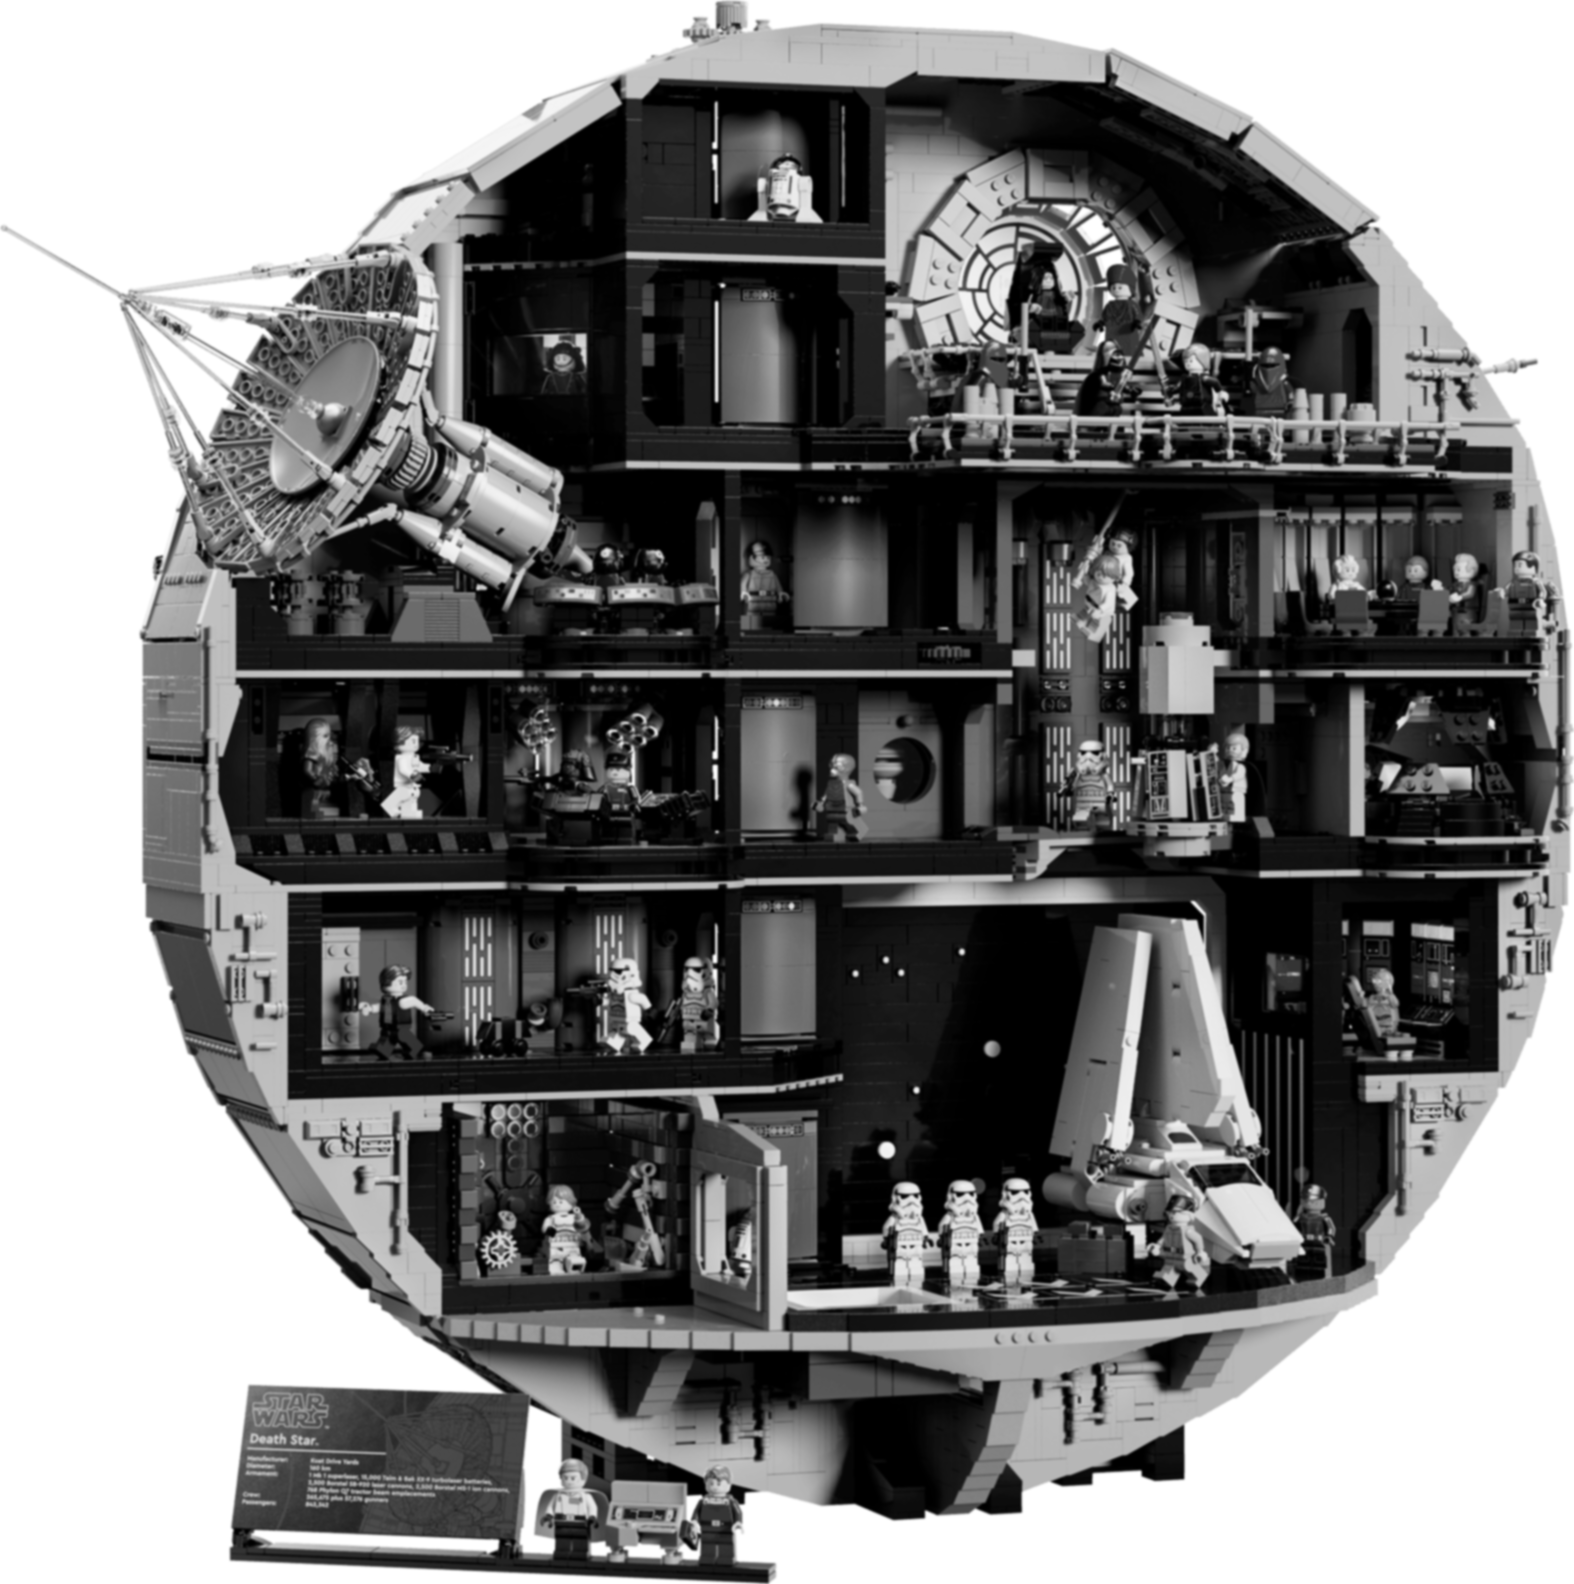
\includegraphics[width=0.45\textwidth]{zad7/oryginal_filtered.png}
\caption{Obraz wejściowy $g$ -- rozmyte zdjęcie \texttt{Lego\_GwiazdaSmierci\_filtered.png}.}
\end{figure}

\begin{figure}[H]
\centering
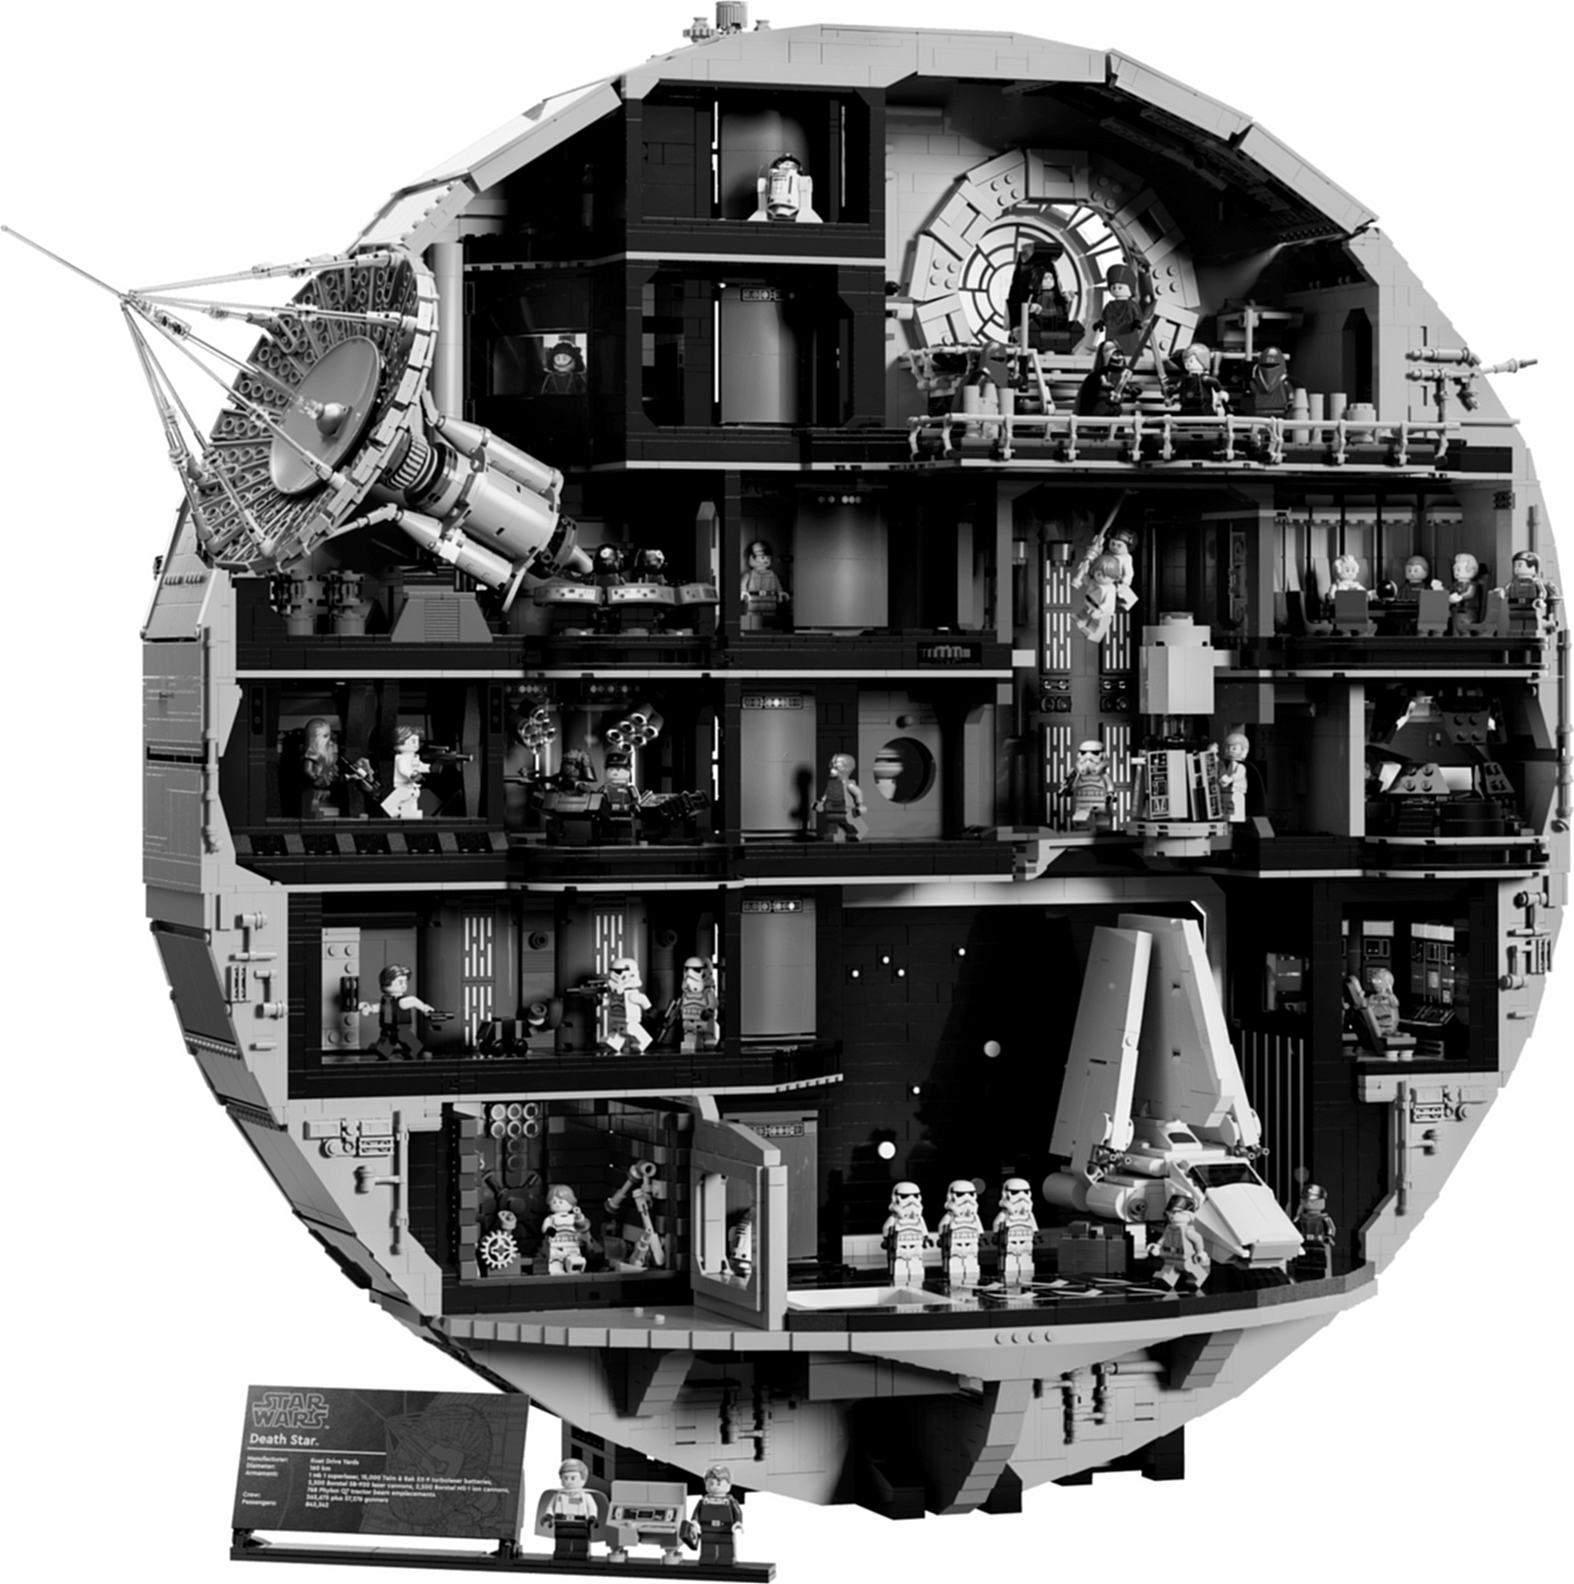
\includegraphics[width=0.45\textwidth]{zad7/dekonwolucja_k2.png}
\caption{Dekonwolucja po $k=2$ iteracjach.}
\end{figure}

\begin{figure}[H]
\centering
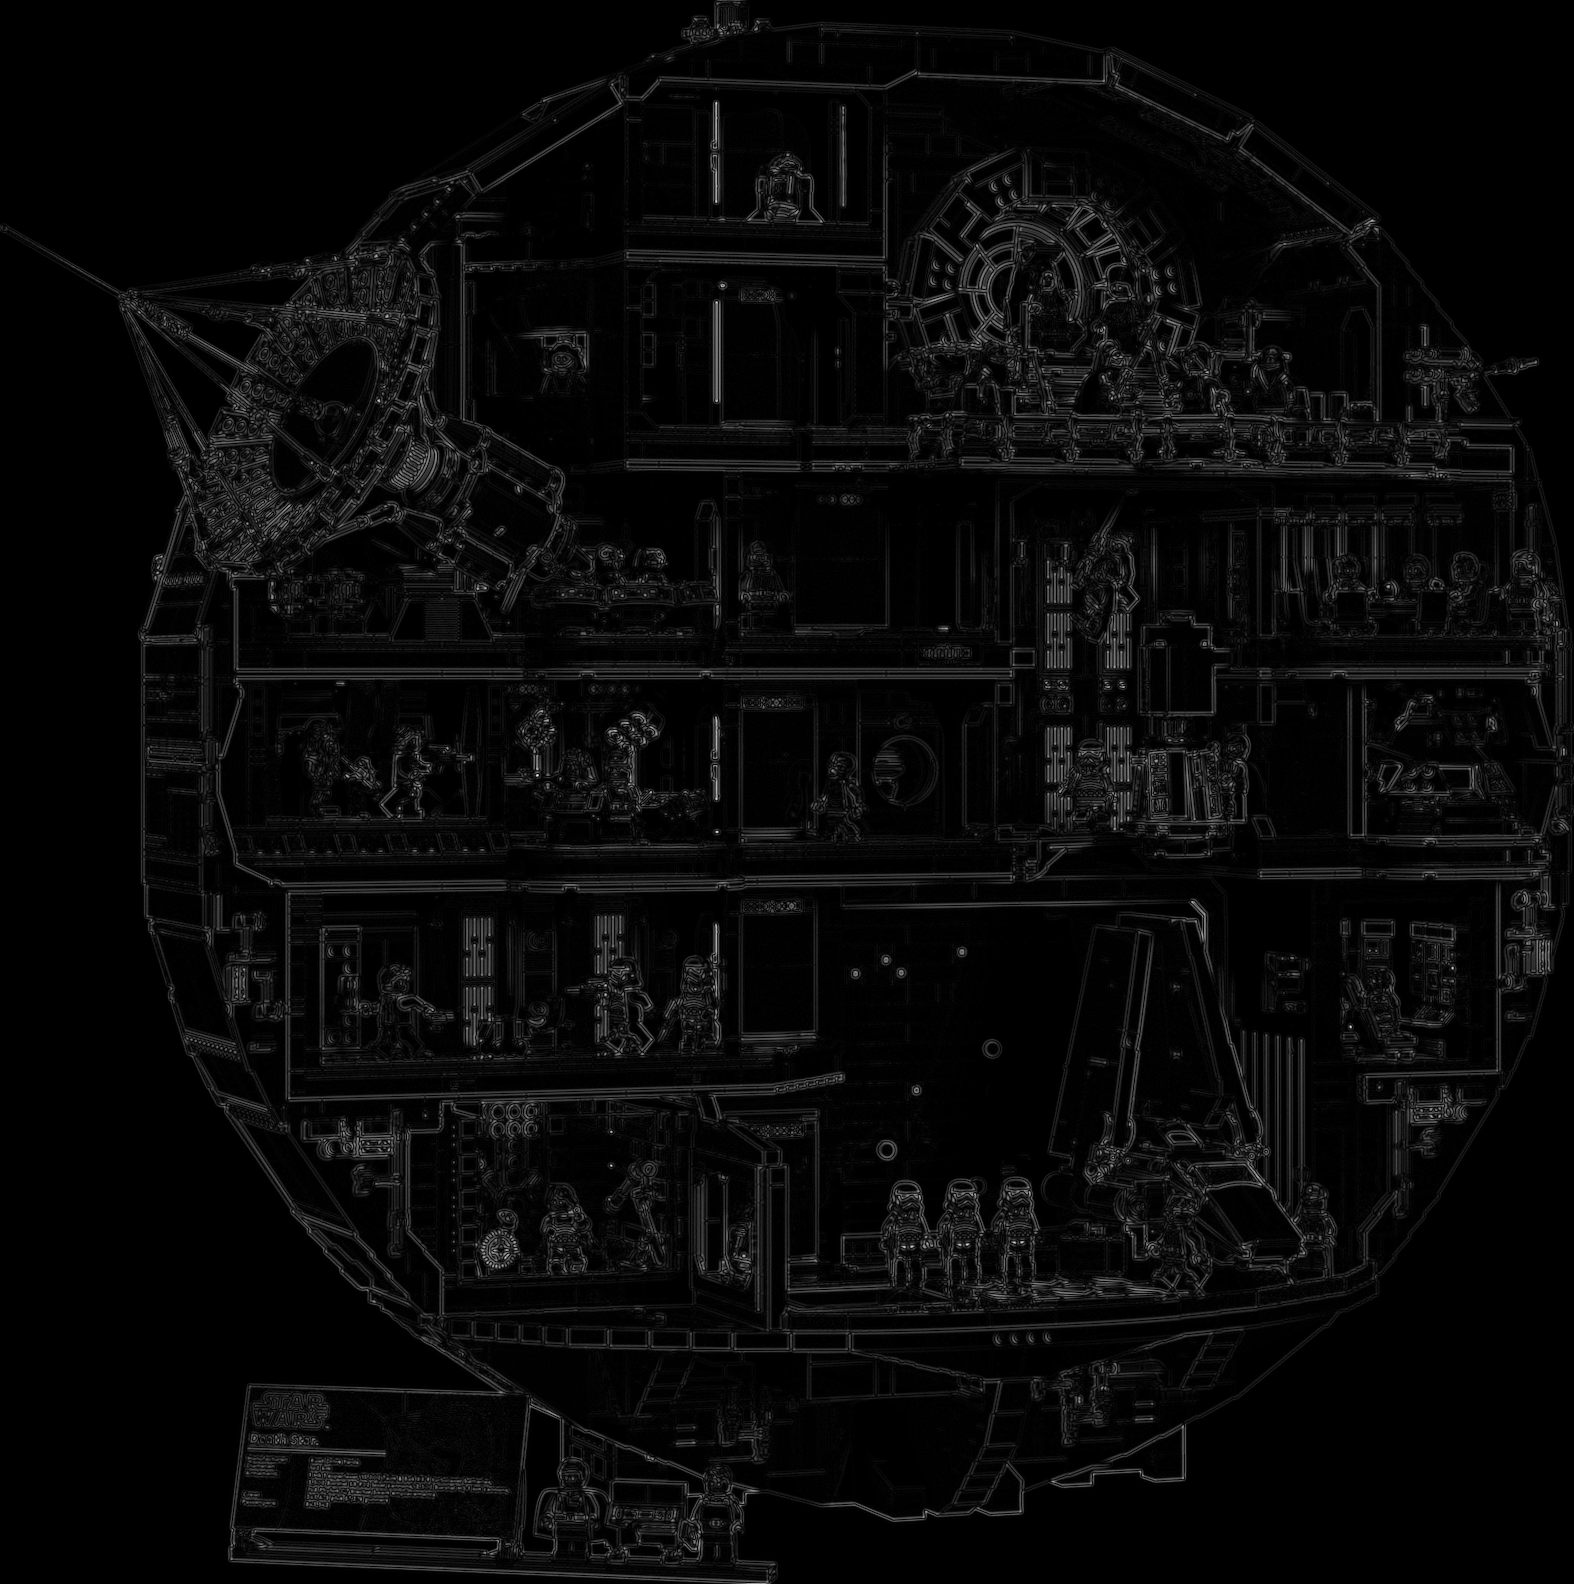
\includegraphics[width=0.45\textwidth]{zad7/roznica_k2.png}
\caption{Różnica symetryczna po $k=2$ iteracjach.}
\end{figure}

\begin{figure}[H]
\centering
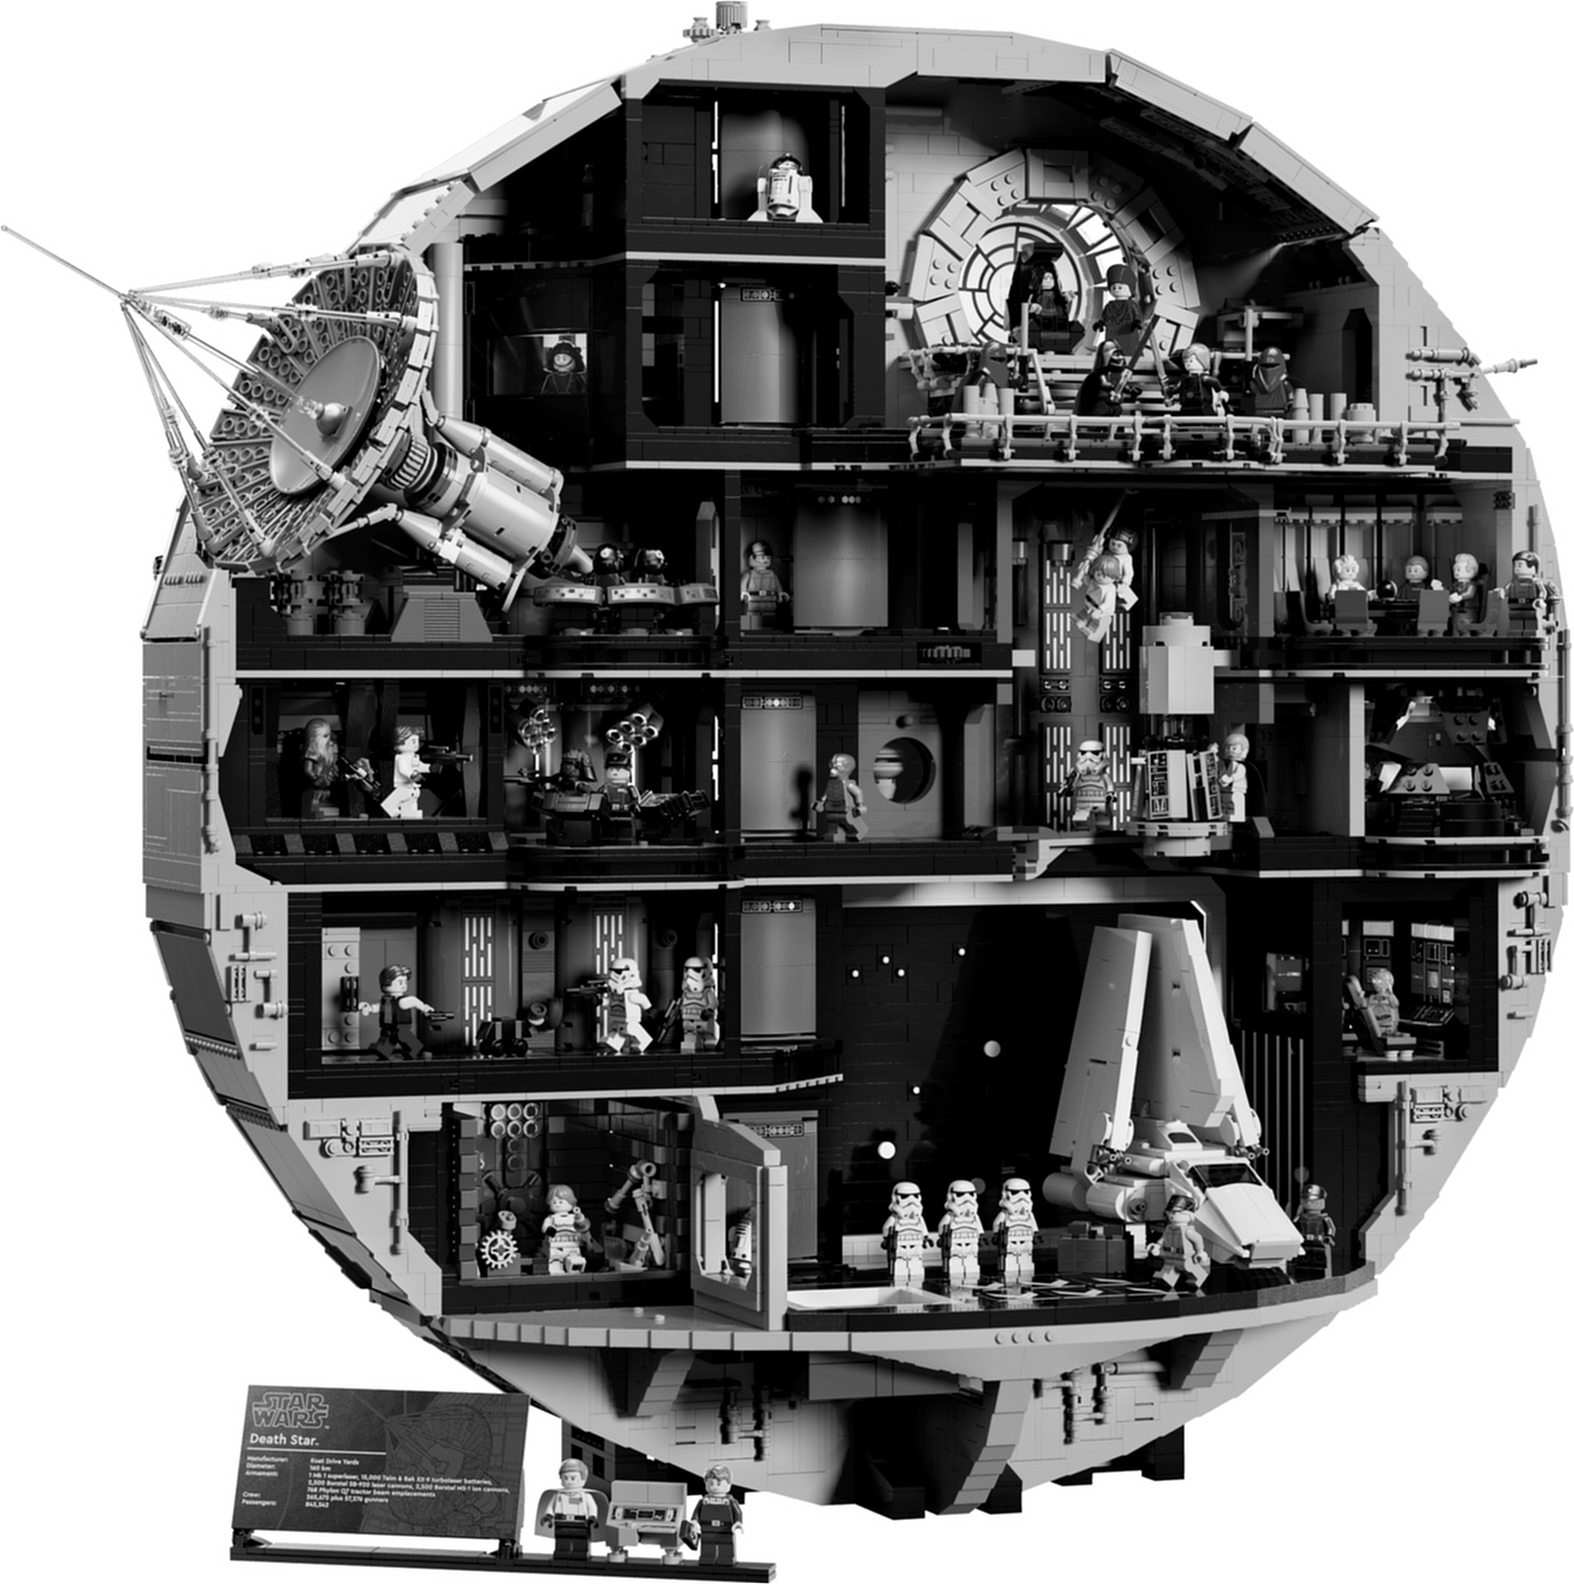
\includegraphics[width=0.45\textwidth]{zad7/dekonwolucja_k5.png}
\caption{Dekonwolucja po $k=5$ iteracjach.}
\end{figure}

\begin{figure}[H]
\centering
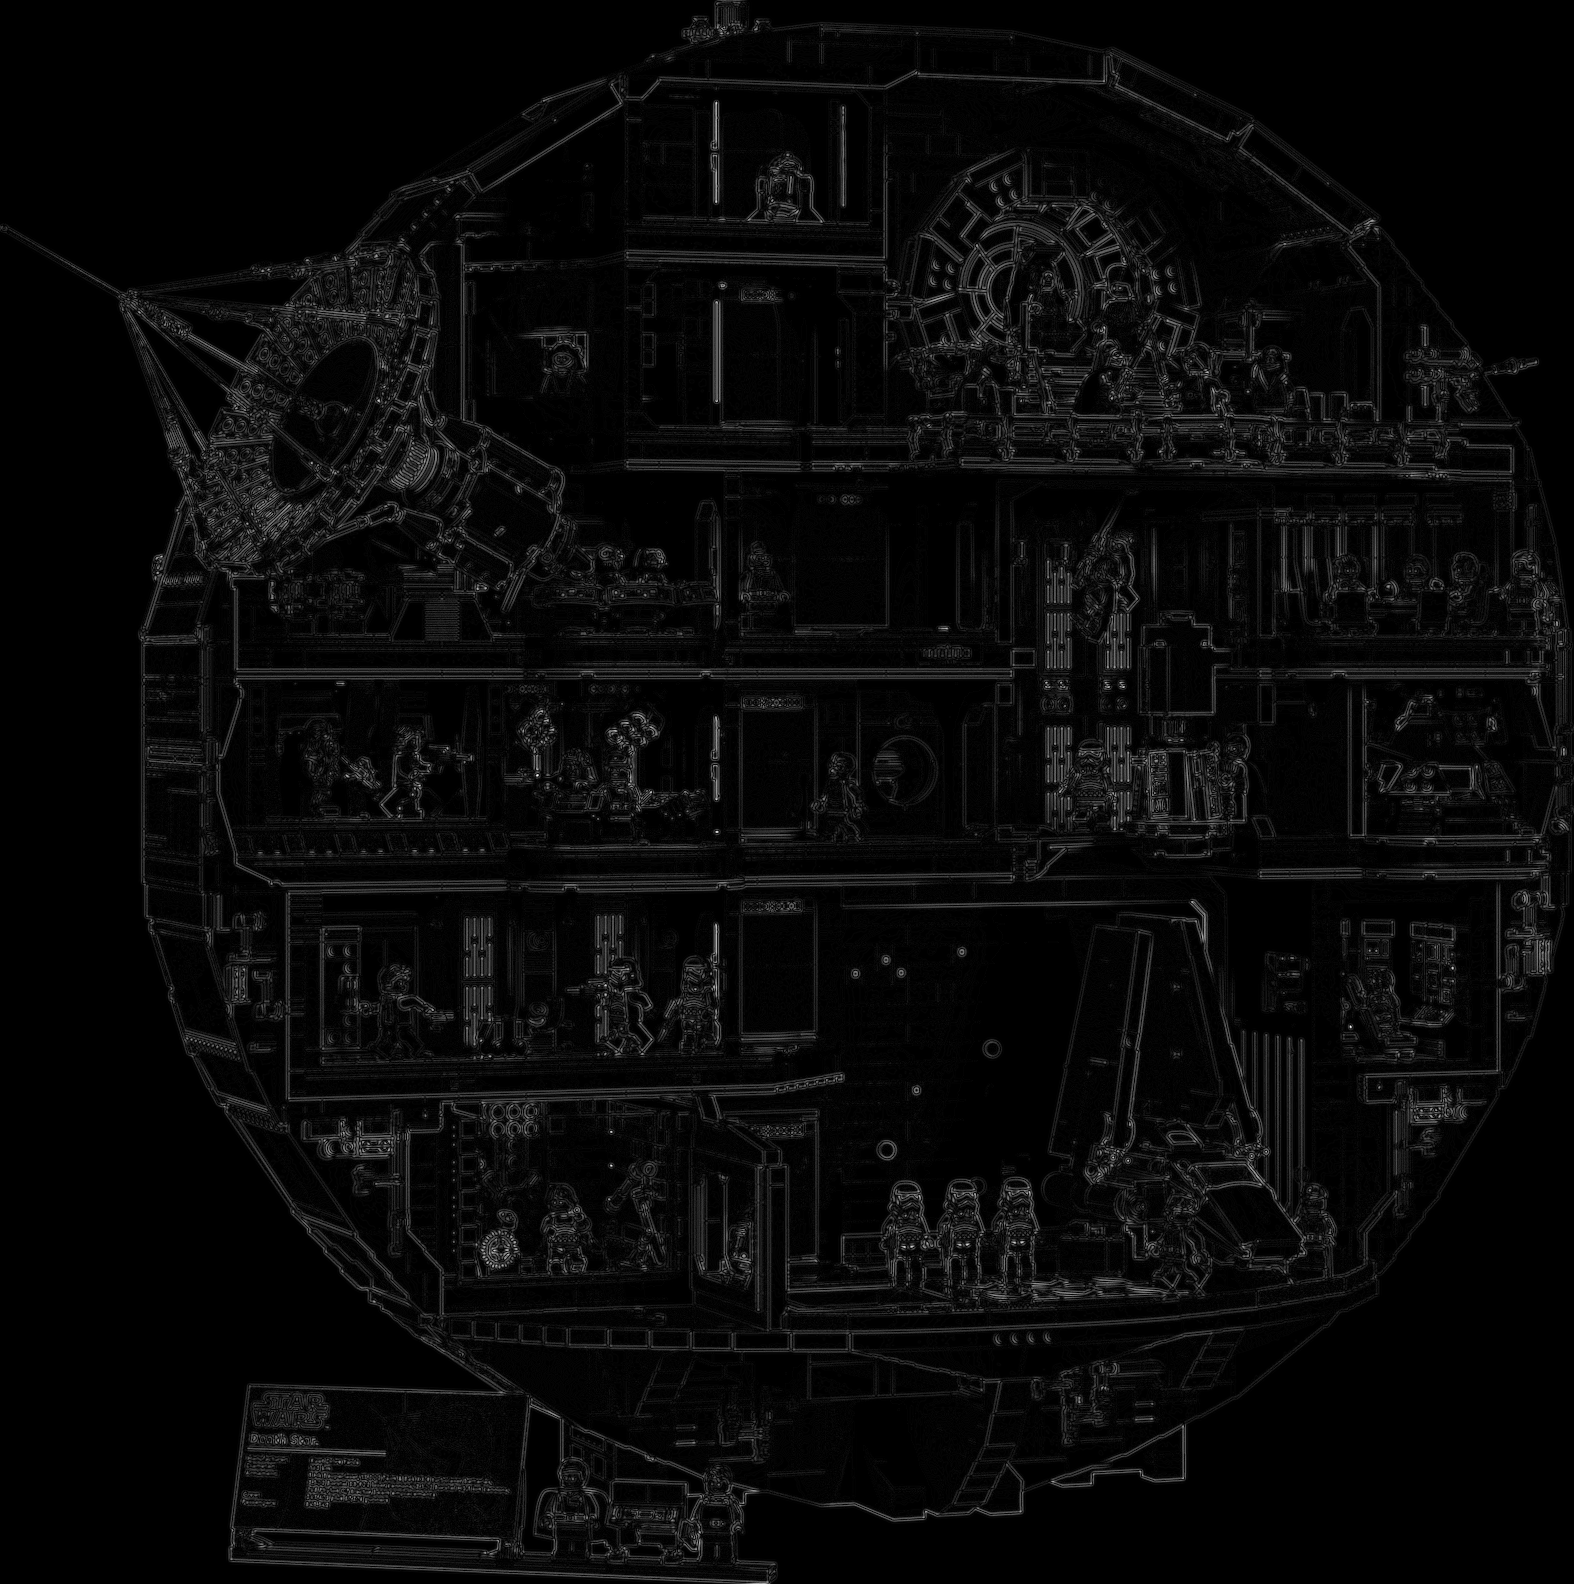
\includegraphics[width=0.45\textwidth]{zad7/roznica_k5.png}
\caption{Różnica symetryczna po $k=5$ iteracjach.}
\end{figure}

\begin{figure}[H]
\centering
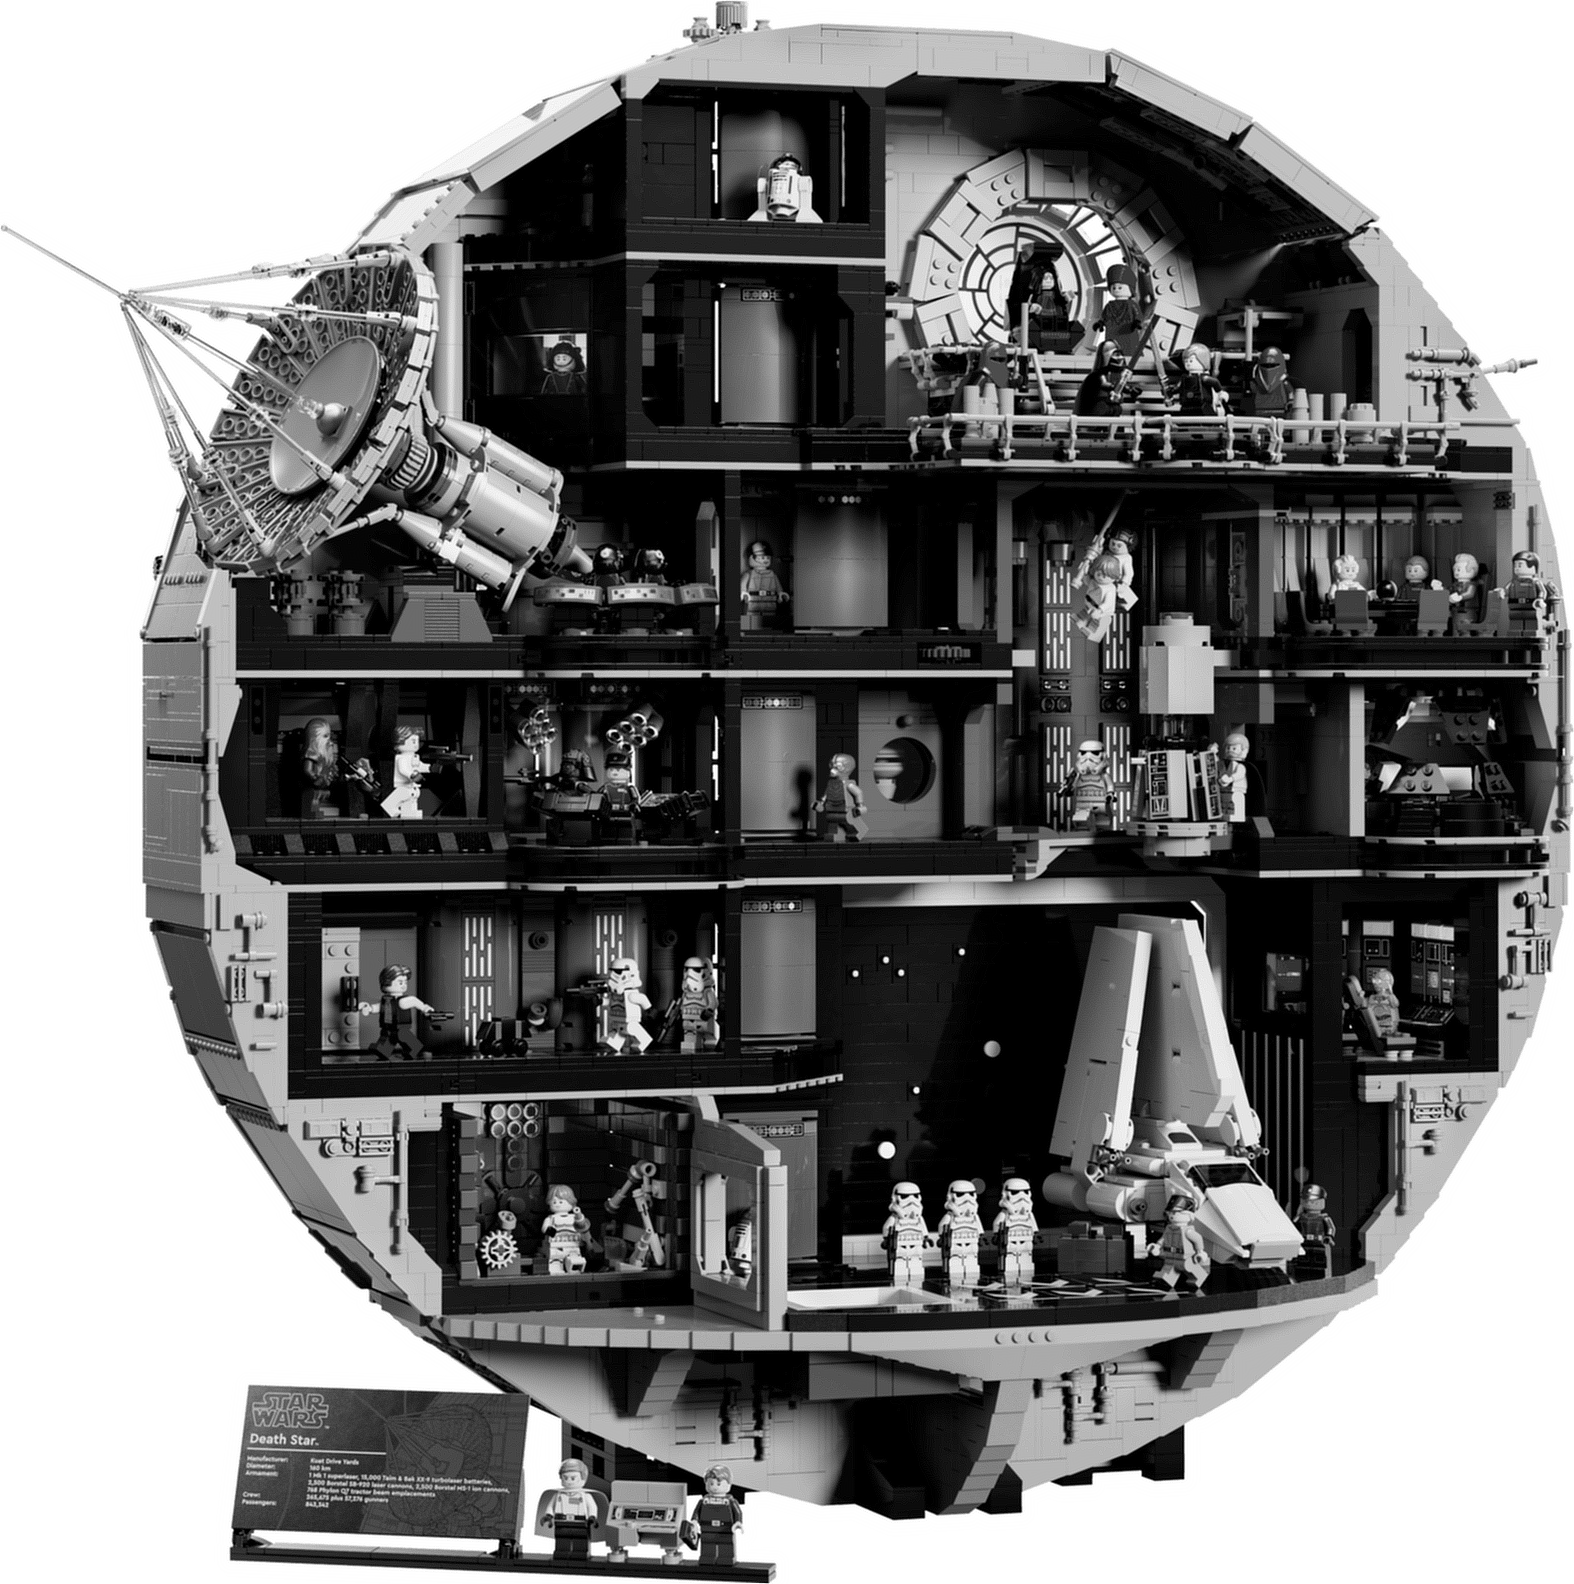
\includegraphics[width=0.45\textwidth]{zad7/dekonwolucja_k15.png}
\caption{Dekonwolucja po $k=15$ iteracjach.}
\end{figure}

\begin{figure}[H]
\centering
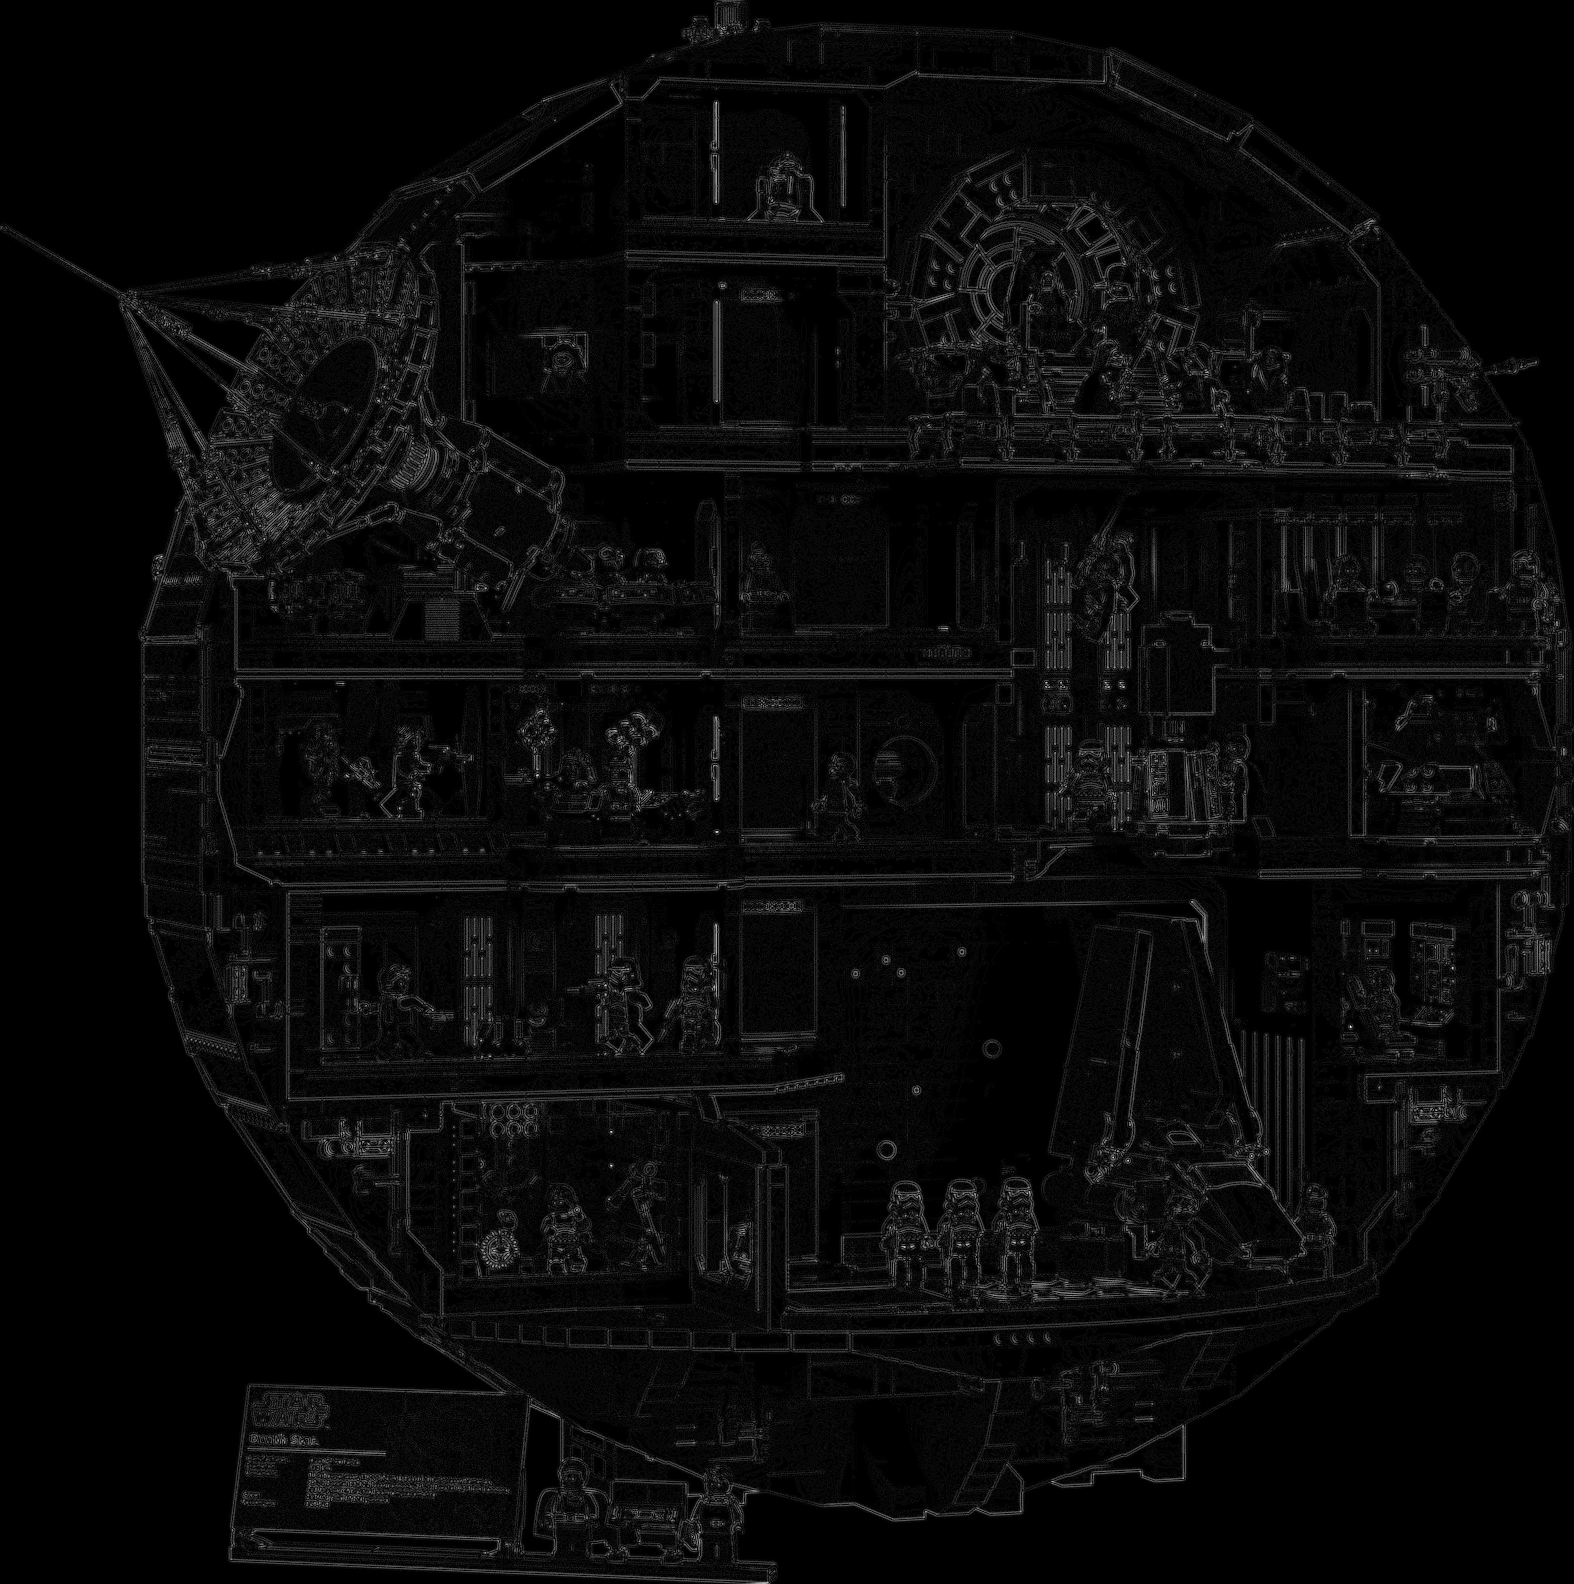
\includegraphics[width=0.45\textwidth]{zad7/roznica_k15.png}
\caption{Różnica symetryczna po $k=15$ iteracjach.}
\end{figure}

\begin{figure}[H]
\centering
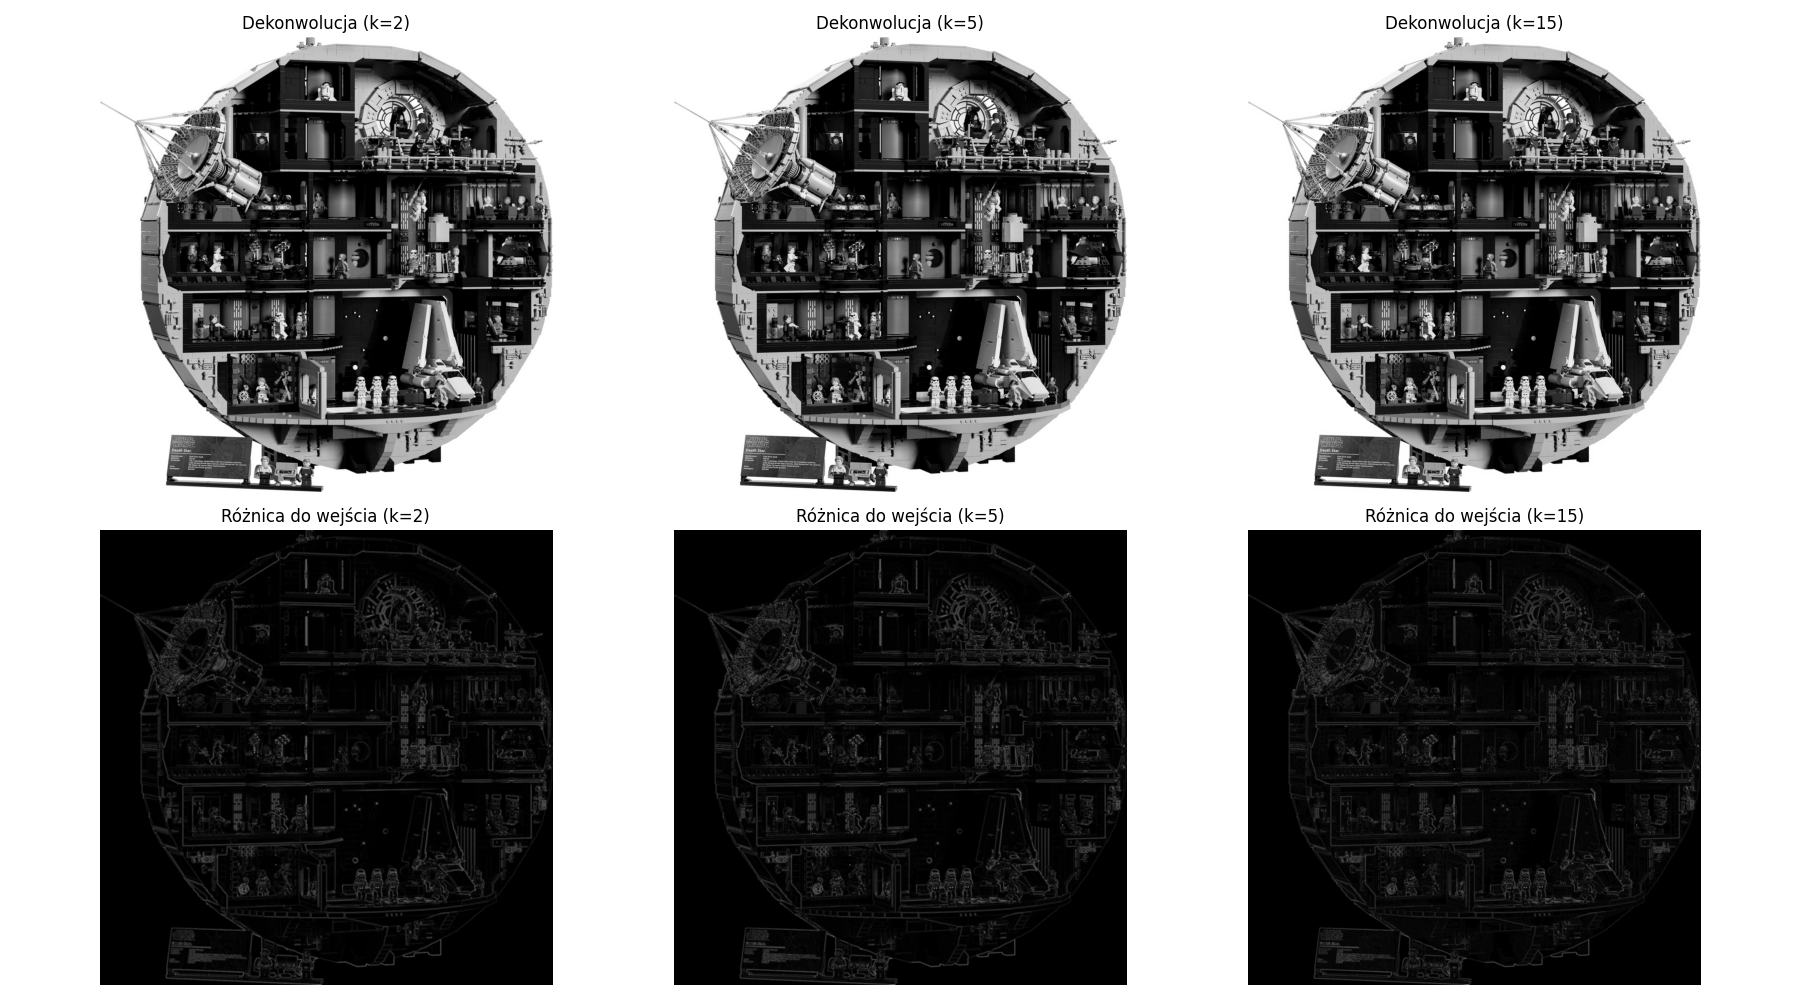
\includegraphics[width=\textwidth]{zad7/zestawienie_van_cittert.png}
\caption{Zestawienie: górny rząd -- wyniki dekonwolucji dla $k=2,5,15$; dolny rząd -- różnice symetryczne względem $g$.}
\end{figure}

\end{document}